\mysection{x86}

\subsection{Терминология}

Общее для 16-bit (8086/80286), 32-bit (80386, итд), 64-bit.

\myindex{IEEE 754}
\myindex{MS-DOS}
\begin{description}
	\item[byte] 8-бит. 
		Для определения переменных и массива байт используется директива ассемблера DB.
		Байты передаются в 8-битных частях регистров: \TT{AL/BL/CL/DL/AH/BH/CH/DH/SIL/DIL/R*L}.
	\item[word] 16-бит. \dittoclosing директива ассемблера DW.
		Слова передаются в 16-битных частях регистров: \\
			\TT{AX/BX/CX/DX/SI/DI/R*W}.
	\item[double word] (\q{dword}) 32-бит. \dittoclosing директива ассемблера DD.
		Двойные слова передаются в регистрах (x86) или в 32-битных частях регистров (x64). 
		В 16-битном коде, двойные слова передаются в парах 16-битных регистров.
	\item[quad word] (\q{qword}) 64-бит. \dittoclosing директива ассемблера DQ.
		В 32-битной среде, учетверенные слова передаются в парах 32-битных регистров.
	\item[tbyte] (10 байт) 80-бит или 10 байт (используется для регистров IEEE 754 FPU).
	\item[paragraph] (16 байт) --- термин был популярен в среде MS-DOS.
\end{description}

\myindex{Windows!API}
Типы данных с той же шириной (BYTE, WORD, DWORD) точно такие же и в Windows \ac{API}.

\subsection{\RU{Регистры общего пользования}\EN{General purpose registers}\DE{Mehrzweckregister}}

\RU{Ко многим регистрам можно обращаться как к частям размером в байт или 16-битное слово}
\EN{It is possible to access many registers by byte or 16-bit word parts}.
\DE{Es ist möglich auf viele Register byteweise oder über 16-Bit-Wortteile zuzugreifen}.

\RU{Это всё --- наследие от более старых процессоров Intel (вплоть до 8-битного 8080),
все еще поддерживаемое для обратной совместимости}\EN{It is all inheritance from older Intel CPUs (up to the 8-bit 8080) 
still supported for backward compatibility}.
\EN{Older 8-bit CPUs (8080) had 16-bit registers divided by two.}
\DE{Ältere 8-Bit-CPUs (8080) hatten 16-Bit-Reigster geteilt durch zwei.}

\RU{Старые 8-битные процессоры 8080 имели 16-битные регистры, разделенные на две части.}
\EN{Programs written for 8080 could access the low byte part of 16-bit registers, high byte part
or the whole 16-bit register.}
\DE{Programme die für den 8080 geschrieben wurden, konnten auf den niederwertigen Teil von
	16-Bit-Registern, den höherwertigen Teil oder auf das ganze 16-Bit-Register zugreifen.}

\RU{Программы, написанные для 8080 имели доступ к младшему байту 16-битного регистра, к старшему
байту или к целому 16-битному регистру.}
\EN{Perhaps, this feature was left in 8086 as a helper for easier porting.}
\DE{Dieses Feature wurde vielleicht als Hilfe für eine einfachere Portierung beim 8086 beibehalten.}

\RU{Вероятно, эта возможность была оставлена в 8086 для более простого портирования.}
\RU{В \ac{RISC} процессорах, такой возможности, как правило, нет}\EN{This feature
is usually not present in \ac{RISC} CPUs}.

\myindex{x86-64}
\RU{Регистры, имеющие префикс \TT{R-} появились только в x86-64, а префикс \TT{E-} ---в 80386.}
\EN{Registers prefixed with \TT{R-} appeared in x86-64, and those prefixed with \TT{E-}---in 80386.}
\DE{Register mit dem Präfix \TT{R-} tauchen bei x86-64 auf; der Präfix \TT{E-}---bei 80386.}

\RU{Таким образом, R-регистры 64-битные, а E-регистры --- 32-битные.}
\EN{Thus, R-registers are 64-bit, and E-registers---32-bit.}
\DE{Dementsprechend sind, R-Register 64-Bit und E-Register 32-Bit.}

\RU{В x86-64 добавили еще 8 \ac{GPR}: R8-R15}
\EN{8 more \ac{GPR}'s were added in x86-86: R8-R15}.
\DE{8 weitere \ac{GPR}'s wurden bei x86-86 hinzugefügt: R8-R15}.

N.B.: \RU{В документации от Intel, для обращения к самому младшему байту к имени регистра
нужно добавлять суффикс \emph{L}: \emph{R8L}, но \ac{IDA} называет эти регистры добавляя суффикс \emph{B}: \emph{R8B}}
\EN{In the Intel manuals the byte parts of these registers are prefixed by \emph{L}, e.g.: \emph{R8L}, but \ac{IDA}
names these registers by adding the \emph{B} suffix, e.g.: \emph{R8B}}.

\subsubsection{RAX/EAX/AX/AL}
\RegTableOne{RAX}{EAX}{AX}{AH}{AL}

\ac{AKA} \RU{аккумулятор}\EN{accumulator}\DE{Akkumulator}.
\RU{Результат функции обычно возвращается через этот регистр}
\EN{The result of a function is usually returned via this register}.
\DE{Das Ergebnis einer Funktion wird in der Regel in einem Register zurückgegeben.}

\subsubsection{RBX/EBX/BX/BL}
\RegTableOne{RBX}{EBX}{BX}{BH}{BL}

\subsubsection{RCX/ECX/CX/CL}
\RegTableOne{RCX}{ECX}{CX}{CH}{CL}

\ac{AKA} \RU{счетчик}\EN{counter}\DE{Zähler}:
\RU{используется в этой роли в инструкциях с префиксом REP и в инструкциях сдвига}
\EN{in this role it is used in REP prefixed instructions and also in shift instructions}
\DE{in dieser Rolle in REP Befehlen und auch als Schiebeoperationen verwendet}
(SHL/SHR/RxL/RxR).

\subsubsection{RDX/EDX/DX/DL}
\RegTableOne{RDX}{EDX}{DX}{DH}{DL}

\subsubsection{RSI/ESI/SI/SIL}
\RegTableTwo{RSI}{ESI}{SI}{SIL}

\ac{AKA} \q{source index}. \RU{Используется как источник в инструкциях}\EN{Used as source in the instructions}
\DE{Als Quelle der Befehle verwendet}
REP MOVSx, REP CMPSx.

\subsubsection{RDI/EDI/DI/DIL}
\RegTableTwo{RDI}{EDI}{DI}{DIL}

\ac{AKA} \q{destination index}. \RU{Используется как указатель на место назначения в инструкции}
\EN{Used as a pointer to the destination in the instructions}
\DE{Als Zeiger auf das Ziel der Befehle verwendet}REP MOVSx, REP STOSx.

% TODO навести тут порядок
\subsubsection{R8/R8D/R8W/R8L}
\RegTableFour{R8}{R8D}{R8W}{R8L}

\subsubsection{R9/R9D/R9W/R9L}
\RegTableFour{R9}{R9D}{R9W}{R9L}

\subsubsection{R10/R10D/R10W/R10L}
\RegTableFour{R10}{R10D}{R10W}{R10L}

\subsubsection{R11/R11D/R11W/R11L}
\RegTableFour{R11}{R11D}{R11W}{R11L}

\subsubsection{R12/R12D/R12W/R12L}
\RegTableFour{R12}{R12D}{R12W}{R12L}

\subsubsection{R13/R13D/R13W/R13L}
\RegTableFour{R13}{R13D}{R13W}{R13L}

\subsubsection{R14/R14D/R14W/R14L}
\RegTableFour{R14}{R14D}{R14W}{R14L}

\subsubsection{R15/R15D/R15W/R15L}
\RegTableFour{R15}{R15D}{R15W}{R15L}

\subsubsection{RSP/ESP/SP/SPL}
\RegTableFour{RSP}{ESP}{SP}{SPL}

\ac{AKA} \gls{stack pointer}. \RU{Обычно всегда указывает на текущий стек, кроме тех случаев,
когда он не инициализирован}\EN{Usually points to the current stack except in those cases when it is not yet initialized}.

\subsubsection{RBP/EBP/BP/BPL}
\RegTableFour{RBP}{EBP}{BP}{BPL}

\ac{AKA} frame pointer. \RU{Обычно используется для доступа к локальным переменным функции и аргументам,
Больше о нем}
\EN{Usually used for local variables and accessing the arguments of the function. More about it}: (\myref{stack_frame}).

\subsubsection{RIP/EIP/IP}

\begin{center}
\begin{tabular}{ | l | l | l | l | l | l | l | l | l |}
\hline
\RegHeaderTop \\
\hline
\RegHeader \\
\hline
\multicolumn{8}{ | c | }{RIP\textsuperscript{x64}} \\
\hline
\multicolumn{4}{ | c | }{} & \multicolumn{4}{ c | }{EIP} \\
\hline
\multicolumn{6}{ | c | }{} & \multicolumn{2}{ c | }{IP} \\
\hline
\end{tabular}
\end{center}

\ac{AKA} \q{instruction pointer}
\footnote{\RU{Иногда называется также}\EN{Sometimes also called} \q{program counter}}.
\RU{Обычно всегда указывает на инструкцию, которая сейчас будет исполняться
Напрямую модифицировать регистр нельзя, хотя можно делать так (что равноценно)}%
\EN{Usually always points to the instruction to be executed right now.
Cannot be modified, however, it is possible to do this (which is equivalent)}:

\begin{lstlisting}
MOV EAX, ...
JMP EAX
\end{lstlisting}

\RU{Либо}\EN{Or}:

\begin{lstlisting}
PUSH value
RET
\end{lstlisting}

\subsubsection{CS/DS/ES/SS/FS/GS}

\RU{16-битные регистры, содержащие селектор кода}\EN{16-bit registers containing code selector} (CS), 
\RU{данных}\EN{data selector} (DS), \RU{стека}\EN{stack selector} (SS).\\
\\
\myindex{TLS}
\myindex{Windows!TIB}
FS \InENRU win32 \RU{указывает на}\EN{points to} \ac{TLS}, \RU{а в Linux на эту роль был выбран GS}
\EN{GS took this role in Linux}.
\RU{Это сделано для более быстрого доступа к \ac{TLS} и прочим структурам там вроде \ac{TIB}}
\EN{It is made so for faster access to the \ac{TLS} and other structures like the \ac{TIB}}.
\\
\RU{В прошлом эти регистры использовались как сегментные регистры}
\EN{In the past, these registers were used as segment registers} (\myref{8086_memory_model}).

\subsubsection{\RU{Регистр флагов}\EN{Flags register}}
\myindex{x86!\Registers!\Flags}
\label{EFLAGS}
\ac{AKA} EFLAGS.

\small
\begin{center}
\begin{tabular}{ | l | l | l | }
\hline
\headercolor{} \RU{Бит}\EN{Bit} (\RU{маска}\EN{mask}) &
\headercolor{} \RU{Аббревиатура}\EN{Abbreviation} (\RU{значение}\EN{meaning}) &
\headercolor{} \RU{Описание}\EN{Description} \\
\hline
0 (1) & CF (Carry) & \RU{Флаг переноса.} \\
      &            & \RU{Инструкции}\EN{The} CLC/STC/CMC \RU{используются}\EN{instructions are used} \\
      &            & \RU{для установки/сброса/инвертирования этого флага}\EN{for setting/resetting/toggling this flag} \\
\hline
2 (4) & PF (Parity) & \RU{Флаг четности }(\myref{parity_flag}). \\
\hline
4 (0x10) & AF (Adjust) & \RU{Существует только для работы с \ac{BCD}-числами}
			\EN{Exist solely for work with \ac{BCD}-numbers} \\
\hline
6 (0x40) & ZF (Zero) & \RU{Выставляется в}\EN{Setting to} 0 \\
         &           & \RU{если результат последней операции был равен}\EN{if the last operation's result is equal to} 0. \\
\hline
7 (0x80) & SF (Sign) & \RU{Флаг знака.} \\
\hline
8 (0x100) & TF (Trap) & \RU{Применяется при отладке}\EN{Used for debugging}. \\
&         &             \RU{Если включен, то после исполнения каждой инструкции}\EN{If turned on, an exception is to be} \\
&         &             \RU{будет сгенерировано исключение}\EN{generated after each instruction's execution}. \\
\hline
9 (0x200) & IF (Interrupt enable) & \RU{Разрешены ли прерывания}\EN{Are interrupts enabled}. \\
          &                       & \RU{Инструкции}\EN{The} CLI/STI \RU{используются}\EN{instructions are used} \\
	  &                       & \RU{для установки/сброса этого флага}\EN{for setting/resetting the flag} \\
\hline
10 (0x400) & DF (Direction) & \RU{Задается направление для инструкций}\EN{A direction is set for the} \\
           &                & REP MOVSx/CMPSx/LODSx/SCASx\EN{ instructions}.\\
           &                & \RU{Инструкции}\EN{The} CLD/STD \RU{используются}\EN{instructions are used} \\
	   &                & \RU{для установки/сброса этого флага}\EN{for setting/resetting the flag} \\
	   &                & \EN{See also}\RU{См.также}: \myref{memmove_and_DF}. \\
\hline
11 (0x800) & OF (Overflow) & \RU{Переполнение.} \\
\hline
12, 13 (0x3000) & IOPL (I/O privilege level)\textsuperscript{i286} & \\
\hline
14 (0x4000) & NT (Nested task)\textsuperscript{i286} & \\
\hline
16 (0x10000) & RF (Resume)\textsuperscript{i386} & \RU{Применяется при отладке}\EN{Used for debugging}. \\
             &                  & \RU{Если включить,}\EN{The CPU ignores the hardware} \\
	     &                  & \RU{CPU проигнорирует хардварную точку останова в DRx}\EN{breakpoint in DRx if the flag is set}. \\
\hline
17 (0x20000) & VM (Virtual 8086 mode)\textsuperscript{i386} & \\
\hline
18 (0x40000) & AC (Alignment check)\textsuperscript{i486} & \\
\hline
19 (0x80000) & VIF (Virtual interrupt)\textsuperscript{i586} & \\
\hline
20 (0x100000) & VIP (Virtual interrupt pending)\textsuperscript{i586} & \\
\hline
21 (0x200000) & ID (Identification)\textsuperscript{i586} & \\
\hline
\end{tabular}
\end{center}
\normalsize

\RU{Остальные флаги зарезервированы}\EN{All the rest flags are reserved}.

\subsection{FPU \registers{}}

\myindex{x86!FPU}
8 80-\RU{битных регистров работающих как стек}\EN{bit registers working as a stack}: ST(0)-ST(7).
N.B.: \ac{IDA} \RU{называет}\EN{calls} ST(0) \RU{просто}\EN{as just} ST.
\RU{Числа хранятся в формате}\EN{Numbers are stored in the} IEEE 754\EN{ format}.

\RU{Формат значения \emph{long double}}\EN{\emph{long double} value format}:

\bigskip
% a hack used here! http://tex.stackexchange.com/questions/73524/bytefield-package
\begin{center}
\begingroup
\makeatletter
\let\saved@bf@bitformatting\bf@bitformatting
\renewcommand*{\bf@bitformatting}{%
	\ifnum\value{header@val}=21 %
	\value{header@val}=62 %
	\else\ifnum\value{header@val}=22 %
	\value{header@val}=63 %
	\else\ifnum\value{header@val}=23 %
	\value{header@val}=64 %
	\else\ifnum\value{header@val}=30 %
	\value{header@val}=78 %
	\else\ifnum\value{header@val}=31 %
	\value{header@val}=79 %
	\fi\fi\fi\fi\fi
	\saved@bf@bitformatting
}%
\begin{bytefield}[bitwidth=0.03\linewidth]{32}
	\bitheader[endianness=big]{0,21,22,23,30,31} \\
	\bitbox{1}{S} &
	\bitbox{8}{\RU{экспонента}\EN{exponent}} &
	\bitbox{1}{I} &
	\bitbox{22}{\RU{мантисса}\EN{mantissa or fraction}}
\end{bytefield}
\endgroup
\end{center}

\begin{center}
( S --- \RU{знак}\EN{sign}, I --- \RU{целочисленная часть}\EN{integer part} )
\end{center}

\label{FPU_control_word}
\subsubsection{\RU{Регистр управления}\EN{Control Word}}

\RU{Регистр, при помощи которого можно задавать поведение}\EN{Register controlling the behavior of the}
\ac{FPU}.

%\small
\begin{center}
\begin{tabular}{ | l | l | l | }
\hline
\RU{Бит}\EN{Bit} &
\RU{Аббревиатура (значение)}\EN{Abbreviation (meaning)} &
\RU{Описание}\EN{Description} \\
\hline
0   & IM (Invalid operation Mask) & \\
\hline
1   & DM (Denormalized operand Mask) & \\
\hline
2   & ZM (Zero divide Mask) & \\
\hline
3   & OM (Overflow Mask) & \\
\hline
4   & UM (Underflow Mask) & \\
\hline
5   & PM (Precision Mask) & \\
\hline
7   & IEM (Interrupt Enable Mask) & \RU{Разрешение исключений, по умолчанию 1 (запрещено)}
\EN{Exceptions enabling, 1 by default (disabled)} \\
\hline
8, 9 & PC (Precision Control) & \RU{Управление точностью} \\
     &                        & 00 ~--- 24 \RU{бита}\EN{bits} (REAL4) \\
     &                        & 10 ~--- 53 \RU{бита}\EN{bits} (REAL8) \\
     &                        & 11 ~--- 64 \RU{бита}\EN{bits} (REAL10) \\
\hline
10, 11 & RC (Rounding Control) & \RU{Управление округлением} \\
       &                       & 00 ~--- \RU{(по умолчанию) округлять к ближайшему}\EN{(by default) round to nearest} \\
       &                       & 01 ~--- \RU{округлять к}\EN{round toward} $-\infty$ \\
       &                       & 10 ~--- \RU{округлять к}\EN{round toward} $+\infty$ \\
       &                       & 11 ~--- \RU{округлять к}\EN{round toward} 0 \\
\hline
12 & IC (Infinity Control) & 0 ~--- (\RU{по умолчанию}\EN{by default}) \RU{считать}\EN{treat} $+\infty$ \AndENRU $-\infty$ \RU{за беззнаковое}\EN{as unsigned} \\
   &                       & 1 ~--- \RU{учитывать и}\EN{respect both} $+\infty$ \AndENRU $-\infty$ \\
\hline
\end{tabular}
\end{center}
%\normalsize

\RU{Флагами}\EN{The} PM, UM, OM, ZM, DM, IM 
\RU{задается, генерировать ли исключения в случае соответствующих ошибок}
\EN{flags define if to generate exception in the case of a corresponding error}.

\subsubsection{\RU{Регистр статуса}\EN{Status Word}}

\label{FPU_status_word}
\RU{Регистр только для чтения}\EN{Read-only register}.

\small
\begin{center}
\begin{tabular}{ | l | l | l | }
\hline
\RU{Бит}\EN{Bit} &
\RU{Аббревиатура (значение)}\EN{Abbreviation (meaning)} &
\RU{Описание}\EN{Description} \\
\hline
15   & B (Busy) & \RU{Работает ли сейчас FPU}\EN{Is FPU do something} (1)
\RU{или закончил и результаты готовы}\EN{or results are ready} (0) \\
\hline
14   & C3 & \\
\hline
13, 12, 11 & TOP & \RU{указывает, какой сейчас регистр является нулевым}
\EN{points to the currently zeroth register} \\
\hline
10 & C2 & \\
\hline
9  & C1 & \\
\hline
8  & C0 & \\
\hline
7  & IR (Interrupt Request) & \\
\hline
6  & SF (Stack Fault) & \\
\hline
5  & P (Precision) & \\
\hline
4  & U (Underflow) & \\
\hline
3  & O (Overflow) & \\
\hline
2  & Z (Zero) & \\
\hline
1  & D (Denormalized) & \\
\hline
0  & I (Invalid operation) & \\
\hline
\end{tabular}
\end{center}
\normalsize

\RU{Биты}\EN{The} SF, P, U, O, Z, D, I \RU{сигнализируют об исключениях}
\EN{bits signal about exceptions}.

\RU{О}\EN{About the} C3, C2, C1, C0 \RU{читайте больше}\EN{you can read more here}: (\myref{Czero_etc}).

N.B.: \RU{когда используется регистр ST(x), FPU прибавляет $x$ к TOP по модулю 8 и получается номер
внутреннего регистра}\EN{When ST(x) is used, the FPU adds $x$ to TOP (by modulo 8) and that is how it gets 
the internal register's number}.

\subsubsection{Tag Word}

\RU{Этот регистр отражает текущее содержимое регистров чисел}
\EN{The register has current information about the usage of numbers registers}.

\begin{center}
\begin{tabular}{ | l | l | l | }
\hline
\RU{Бит}\EN{Bit} & \RU{Аббревиатура (значение)}\EN{Abbreviation (meaning)} \\
\hline
15, 14 & Tag(7) \\
\hline
13, 12 & Tag(6) \\
\hline
11, 10 & Tag(5) \\
\hline
9, 8 & Tag(4) \\
\hline
7, 6 & Tag(3) \\
\hline
5, 4 & Tag(2) \\
\hline
3, 2 & Tag(1) \\
\hline
1, 0 & Tag(0) \\
\hline
\end{tabular}
\end{center}

\EN{Each tag contains information about a physical FPU register (R(x)), not logical (ST(x)).}
\RU{Каждый тэг содержит информацию о физическом регистре FPU (R(x)), но не логическом (ST(x)).}

\RU{Для каждого тэга}\EN{For each tag}:

\begin{itemize}
\item 00 ~--- \RU{Регистр содержит ненулевое значение}\EN{The register contains a non-zero value}
\item 01 ~--- \RU{Регистр содержит 0}\EN{The register contains 0}
\EN{\item 10 ~--- The register contains a special value (\ac{NAN}, $\infty$, or denormal)}
\RU{\item 10 ~--- Регистр содержит специальное число (\ac{NAN}, $\infty$, или денормализованное число)}
\item 11 ~--- \RU{Регистр пуст}\EN{The register is empty}
\end{itemize}

\subsection{SIMD \registers{}}

\subsubsection{MMX \registers{}}

8 64-\RU{битных регистров}\EN{bit registers}: MM0..MM7.

\subsubsection{SSE \AndENRU AVX \registers{}}

\myindex{x86-64}
SSE: 8 128-\RU{битных регистров}\EN{bit registers}\DE{Bit-Register}: XMM0..XMM7.
\RU{В}\EN{In the} x86-64 \RU{добавлено еще 8 регистров}\EN{8 more registers were added}: XMM8..XMM15.

AVX \RU{это расширение всех регистры до 256 бит}
\EN{is the extension of all these registers to 256 bits}
\DE{ist eine Erweiterung aller Register auf 256 Bit}.

\subsection{\RU{Отладочные регистры}\EN{Debugging registers}}

\RU{Применяются для работы с т.н.}\EN{Used for} hardware breakpoints\EN{ control}.

\begin{itemize}
	\item DR0 --- \RU{адрес точки останова}\EN{address of breakpoint} \#1
	\item DR1 --- \RU{адрес точки останова}\EN{address of breakpoint} \#2
	\item DR2 --- \RU{адрес точки останова}\EN{address of breakpoint} \#3
	\item DR3 --- \RU{адрес точки останова}\EN{address of breakpoint} \#4
	\item DR6 --- \RU{здесь отображается причина останова}\EN{a cause of break is reflected here}
	\item DR7 --- \RU{здесь можно задать типы точек останова}\EN{breakpoint types are set here}
\end{itemize}

\subsubsection{DR6}
\myindex{x86!\Registers!DR6}

\begin{center}
\begin{tabular}{ | l | l | }
\hline
\headercolor\ \RU{Бит}\EN{Bit} (\RU{маска}\EN{mask}) &
\headercolor\ \RU{Описание}\EN{Description} \\
\hline
0 (1)       &  B0 --- \RU{сработала точка останова \#1}\EN{breakpoint \#1 has been triggered} \\
\hline
1 (2)       &  B1 --- \RU{сработала точка останова \#2}\EN{breakpoint \#2 has been triggered} \\
\hline
2 (4)       &  B2 --- \RU{сработала точка останова \#3}\EN{breakpoint \#3 has been triggered} \\
\hline
3 (8)       &  B3 --- \RU{сработала точка останова \#4}\EN{breakpoint \#4 has been triggered} \\
\hline
13 (0x2000) &  BD --- \RU{была попытка модифицировать один из регистров DRx.}
               \EN{modification attempt of one of the DRx registers.} \\
            &  \RU{может быть выставлен если бит GD выставлен.}
	       \EN{may be raised if GD is enabled} \\
\hline
14 (0x4000) &  BS --- \RU{точка останова типа single step (флаг TF был выставлен в EFLAGS)}
               \EN{single step breakpoint (TF flag has been set in EFLAGS)}. \\
	    &  \RU{Наивысший приоритет. Другие биты также могут быть выставлены}
	       \EN{Highest priority. Other bits may also be set}. \\
\hline
% TODO: describe BT
15 (0x8000) &  BT (task switch flag) \\
\hline
\end{tabular}
\end{center}

N.B. \RU{Точка останова single step это срабатывающая после каждой инструкции}
\EN{A single step breakpoint is a breakpoint which occurs after each instruction}.
\RU{Может быть включена выставлением флага TF в EFLAGS}
\EN{It can be enabled by setting TF in EFLAGS} (\myref{EFLAGS}).

\subsubsection{DR7}
\myindex{x86!\Registers!DR7}

\RU{В этом регистре задаются типы точек останова}\EN{Breakpoint types are set here}.

%\small
\begin{center}
\begin{tabular}{ | l | l | }
\hline
\headercolor\ \RU{Бит}\EN{Bit} (\RU{маска}\EN{mask}) &
\headercolor\ \RU{Описание}\EN{Description} \\
\hline
0 (1)       &  L0 --- \RU{разрешить точку останова}\EN{enable breakpoint} \#1 \RU{для текущей задачи}\EN{for the current task} \\
\hline
1 (2)       &  G0 --- \RU{разрешить точку останова}\EN{enable breakpoint} \#1 \RU{для всех задач}\EN{for all tasks} \\
\hline
2 (4)       &  L1 --- \RU{разрешить точку останова}\EN{enable breakpoint} \#2 \RU{для текущей задачи}\EN{for the current task} \\
\hline
3 (8)       &  G1 --- \RU{разрешить точку останова}\EN{enable breakpoint} \#2 \RU{для всех задач}\EN{for all tasks} \\
\hline
4 (0x10)    &  L2 --- \RU{разрешить точку останова}\EN{enable breakpoint} \#3 \RU{для текущей задачи}\EN{for the current task} \\
\hline
5 (0x20)    &  G2 --- \RU{разрешить точку останова}\EN{enable breakpoint} \#3 \RU{для всех задач}\EN{for all tasks} \\
\hline
6 (0x40)    &  L3 --- \RU{разрешить точку останова}\EN{enable breakpoint} \#4 \RU{для текущей задачи}\EN{for the current task} \\
\hline
7 (0x80)    &  G3 --- \RU{разрешить точку останова}\EN{enable breakpoint} \#4 \RU{для всех задач}\EN{for all tasks} \\
\hline
8 (0x100)   &  LE --- \RU{не поддерживается, начиная с P6}\EN{not supported since P6} \\
\hline
9 (0x200)   &  GE --- \RU{не поддерживается, начиная с P6}\EN{not supported since P6} \\
\hline
13 (0x2000) &  GD --- \RU{исключение будет вызвано если какая-либо инструкция MOV}
			\EN{exception is to be raised if any MOV instruction} \\
            & \RU{попытается модифицировать один из DRx-регистров}
			\EN{tries to modify one of the DRx registers} \\
\hline
16,17 (0x30000)    &  \RU{точка останова}\EN{breakpoint} \#1: R/W --- \RU{тип}\EN{type} \\
\hline
18,19 (0xC0000)    &  \RU{точка останова}\EN{breakpoint} \#1: LEN --- \RU{длина}\EN{length} \\
\hline
20,21 (0x300000)   &  \RU{точка останова}\EN{breakpoint} \#2: R/W --- \RU{тип}\EN{type} \\
\hline
22,23 (0xC00000)   &  \RU{точка останова}\EN{breakpoint} \#2: LEN --- \RU{длина}\EN{length} \\
\hline
24,25 (0x3000000)  &  \RU{точка останова}\EN{breakpoint} \#3: R/W --- \RU{тип}\EN{type} \\
\hline
26,27 (0xC000000)  &  \RU{точка останова}\EN{breakpoint} \#3: LEN --- \RU{длина}\EN{length} \\
\hline
28,29 (0x30000000) &  \RU{точка останова}\EN{breakpoint} \#4: R/W --- \RU{тип}\EN{type} \\
\hline
30,31 (0xC0000000) &  \RU{точка останова}\EN{breakpoint} \#4: LEN --- \RU{длина}\EN{length} \\
\hline
\end{tabular}
\end{center}
%\normalsize

\RU{Так задается тип точки останова}\EN{The breakpoint type is to be set as follows} (R/W):

\begin{itemize}
\item 00 --- \RU{исполнение инструкции}\EN{instruction execution}
\item 01 --- \RU{запись в память}\EN{data writes}
\item 10 --- \RU{обращения к I/O-портам (недоступно из user-mode)}\EN{I/O reads or writes (not available in user-mode)}
\item 11 --- \RU{обращение к памяти (чтение или запись)}\EN{on data reads or writes}
\end{itemize}

N.B.: \RU{отдельного типа для чтения из памяти действительно нет}
\EN{breakpoint type for data reads is absent, indeed}. \\
\\
\RU{Так задается длина точки останова}\EN{Breakpoint length is to be set as follows} (LEN):

\begin{itemize}
\item 00 --- \RU{1 байт}\EN{one-byte}
\item 01 --- \RU{2 байта}\EN{two-byte}
\item 10 --- \RU{не определено для 32-битного режима, 8 байт для 64-битного}
		\EN{undefined for 32-bit mode, eight-byte in 64-bit mode}
\item 11 --- \RU{4 байта}\EN{four-byte}
\end{itemize}


% TODO: control registers
 % subsection
\subsection{\RU{Инструкции}\EN{Instructions}}
\label{sec:x86_instructions}

\RU{Инструкции, отмеченные как (M) обычно не генерируются компилятором: если вы видите её, очень может быть
это вручную написанный фрагмент кода, либо это т.н. compiler intrinsic}
\EN{Instructions marked as (M) are not usually generated by the compiler: if you see one of them, it is probably
a hand-written piece of assembly code, or a compiler intrinsic} (\myref{sec:compiler_intrinsic}).

% TODO ? обратные инструкции

\RU{Только наиболее используемые инструкции перечислены здесь}
\EN{Only the most frequently used instructions are listed here}.
\EN{You can read \myref{x86_manuals} for a full documentation.}%
\RU{Обращайтесь к \myref{x86_manuals} для полной документации.}

\RU{Нужно ли заучивать опкоды инструкций на память?}\EN{Do you have to know all instruction's opcodes by heart?}
\RU{Нет, только те, которые часто используются для модификации кода}\EN{No, only those
which are used for code patching} (\myref{x86_patching}).
\RU{Остальные запоминать нет смысла.}\EN{All the rest of the opcodes don't need to be memorized.}

\subsubsection{\RU{Префиксы}\EN{Prefixes}}

\myindex{x86!\Prefixes!LOCK}
\myindex{x86!\Prefixes!REP}
\myindex{x86!\Prefixes!REPE/REPNE}
\begin{description}
\label{x86_lock}
\item[LOCK] \RU{используется чтобы предоставить эксклюзивный доступ к памяти в многопроцессорной среде}
\EN{forces CPU to make exclusive access to the RAM in multiprocessor environment}.
\RU{Для упрощения, можно сказать, что когда исполняется инструкция с этим префиксом, остальные процессоры
в системе останавливаются}\EN{For the sake of simplification, it can be said that when an instruction
with this prefix is executed, all other CPUs in a multiprocessor system are stopped}.
\RU{Чаще все это используется для критических секций, семафоров, мьютексов}\EN{Most often
it is used for critical sections, semaphores, mutexes}.
\RU{Обычно используется с}\EN{Commonly used with} ADD, AND, BTR, BTS, CMPXCHG, OR, XADD, XOR.
\RU{Читайте больше о критических секциях}\EN{You can read more about critical sections here} (\myref{critical_sections}).

\item[REP] \RU{используется с инструкциями}\EN{is used with the} MOVSx \AndENRU STOSx\EN{ instructions}:
\RU{инструкция будет исполняться в цикле, счетчик расположен в регистре CX/ECX/RCX}
\EN{execute the instruction in a loop, the counter is located in the CX/ECX/RCX register}.
\RU{Для более детального описания, читайте больше об инструкциях}
\EN{For a detailed description, read more about the} MOVSx (\myref{REP_MOVSx}) 
\AndENRU STOSx (\myref{REP_STOSx})\EN{ instructions}.

\RU{Работа инструкций с префиксом REP зависит от флага DF, он задает направление}
\EN{The instructions prefixed by REP are sensitive to the DF flag, which is used to set the direction}.

\item[REPE/REPNE] (\ac{AKA} REPZ/REPNZ) \RU{используется с инструкциями}\EN{used with} CMPSx \AndENRU
SCASx\EN{ instructions}:
\RU{инструкция будет исполняться в цикле, счетчик расположен в регистре \TT{CX}/\TT{ECX}/\TT{RCX}}
\EN{execute the last instruction in a loop, the count is set in the \TT{CX}/\TT{ECX}/\TT{RCX} register}. 
\RU{Выполнение будет прервано если ZF будет 0 (REPE) либо если ZF будет 1 (REPNE)}
\EN{It terminates prematurely if ZF is 0 (REPE) or if ZF is 1 (REPNE)}.

\RU{Для более детального описания, читайте больше об инструкциях}
\EN{For a detailed description, you can read more about the} CMPSx (\myref{REPE_CMPSx}) 
\AndENRU SCASx (\myref{REPNE_SCASx})\EN{ instructions}.

\RU{Работа инструкций с префиксами REPE/REPNE зависит от флага DF, он задает направление}
\EN{Instructions prefixed by REPE/REPNE are sensitive to the DF flag, which is used to set the direction}.

\end{description}

\subsubsection{\RU{Наиболее часто используемые инструкции}\EN{Most frequently used instructions}}

\RU{Их можно заучить в первую очередь}\EN{These can be memorized in the first place}.

\begin{description}
% in order to keep them easily sorted...
\myindex{x86!\Instructions!ADC}
\myindex{x86!\Flags!CF}
  \item[ADC] (\emph{add with carry}) \RU{сложить два значения, \glslink{increment}{инкремент} 
  если выставлен флаг CF.
  ADC часто используется для складывания больших значений, например, складывания двух 64-битных
  значений в 32-битной среде используя две инструкции ADD и ADC, например:}
  \EN{add values, \gls{increment} the result if the CF flag is set.
  ADC is often used for the addition of large values, for example, 
  to add two 64-bit values in a 32-bit environment using two ADD and ADC instructions. For example:}

\EN{\lstinputlisting[style=customasmx86]{appendix/x86/instructions/ADC_example_EN.lst}}
\RU{\lstinputlisting[style=customasmx86]{appendix/x86/instructions/ADC_example_RU.lst}}

\RU{Еще один пример}\EN{One more example}: \myref{sec:64bit_in_32_env}.

\myindex{x86!\Instructions!ADD}
  \item[ADD] \RU{сложить два значения}\EN{add two values}\FR{ajoute deux valeurs}

\myindex{x86!\Instructions!AND}
  \item[AND] \RU{логическое \q{И}}\EN{logical \q{and}}\FR{\q{et} logique}

\myindex{x86!\Instructions!CALL}
  \item[CALL] \RU{вызвать другую функцию}\EN{call another function}\FR{appelle une autre fonction}:\\
  \TT{PUSH address\_after\_CALL\_instruction; JMP label}

\myindex{x86!\Instructions!CMP}
\myindex{x86!\Instructions!SUB}
  \item[CMP] \RU{сравнение значений и установка флагов, то же что и \TT{SUB}, но только без записи результата}
  \EN{compare values and set flags, the same as \TT{SUB} but without writing the result}
  \FR{compare les valeurs et met les flags, comme \TT{SUB} mais sans écrire le résultat}

\myindex{x86!\Instructions!DEC}
\myindex{x86!\Flags!CF}
  \item[DEC] \gls{decrement}.
\RU{В отличие от других арифметических инструкций, \TT{DEC} не модифицирует флаг CF.}%
\EN{Unlike other arithmetic instructions, \TT{DEC} doesn't modify CF flag.}%
\FR{Contrairement aux autres instructions arithmétiques, \TT{DEC} ne modifie pas
le flag CF.}

\myindex{x86!\Instructions!IMUL}
  \item[IMUL] \RU{умножение с учетом знаковых значений}\EN{signed multiply}\FR{multiplication signée}
  \EN{\IMUL often used instead of \MUL, read more about it:}%
  \RU{\IMUL часто используется вместо \MUL, читайте об этом больше:}%
  \FR{\IMUL est souvent utilisé à la place de \MUL, voir ici:} \ref{IMUL_over_MUL}.


\myindex{x86!\Instructions!INC}
\myindex{x86!\Flags!CF}
  \item[INC] \gls{increment}.
\RU{В отличие от других арифметических инструкций, \TT{INC} не модифицирует флаг CF.}%
\EN{Unlike other arithmetic instructions, \TT{INC} doesn't modify CF flag.}

\myindex{x86!\Instructions!JCXZ}
\myindex{x86!\Instructions!JECXZ}
\myindex{x86!\Instructions!JRCXZ}
  \item[JCXZ, JECXZ, JRCXZ] (M) \RU{переход если CX/ECX/RCX=0}\EN{jump if CX/ECX/RCX=0}\FR{saute si CX/ECX/RCX=0}

\myindex{x86!\Instructions!JMP}
\item[JMP] \RU{перейти на другой адрес}\EN{jump to another address}\FR{saute à une
autre adresse}.
\RU{Опкод имеет т.н.}\EN{The opcode has a}\FR{L'opcode a un} \gls{jump offset}.

\item[Jcc] (\RU{где}\EN{where} cc --- condition code)

\myindex{x86!\Instructions!JAE}
\myindex{x86!\Instructions!JA}
\myindex{x86!\Instructions!JBE}
\myindex{x86!\Instructions!JB}
\myindex{x86!\Instructions!JC}
\myindex{x86!\Instructions!JE}
\myindex{x86!\Instructions!JGE}
\myindex{x86!\Instructions!JG}
\myindex{x86!\Instructions!JLE}
\myindex{x86!\Instructions!JL}
\myindex{x86!\Instructions!JNAE}
\myindex{x86!\Instructions!JNA}
\myindex{x86!\Instructions!JNBE}
\myindex{x86!\Instructions!JNB}
\myindex{x86!\Instructions!JNC}
\myindex{x86!\Instructions!JNE}
\myindex{x86!\Instructions!JNGE}
\myindex{x86!\Instructions!JNG}
\myindex{x86!\Instructions!JNLE}
\myindex{x86!\Instructions!JNL}
\myindex{x86!\Instructions!JNO}
\myindex{x86!\Instructions!JNS}
\myindex{x86!\Instructions!JNZ}
\myindex{x86!\Instructions!JO}
\myindex{x86!\Instructions!JPO}
\myindex{x86!\Instructions!JP}
\myindex{x86!\Instructions!JS}
\myindex{x86!\Instructions!JZ}

\RU{Немало этих инструкций имеют синонимы (отмечены с AKA), это сделано для удобства}
\EN{A lot of these instructions have synonyms (denoted with AKA), this was done for convenience}.
\RU{Синонимичные инструкции транслируются в один и тот же опкод}
\EN{Synonymous instructions are translated into the same opcode}.
\RU{Опкод имеет т.н.}\EN{The opcode has a} \gls{jump offset}.

\label{Jcc}
\begin{description}
\item[JAE] \ac{AKA} JNC: \RU{переход если больше или равно (беззнаковый)}\EN{jump if above or equal (unsigned)}: CF=0
\EN{\item[JA] \ac{AKA} JNBE: jump if greater (unsigned): CF=0 and ZF=0}
\RU{\item[JA] \ac{AKA} JNBE: переход если больше (беззнаковый): CF=0 и ZF=0}
\EN{\item[JBE] jump if lesser or equal (unsigned): CF=1 or ZF=1}
\RU{\item[JBE] переход если меньше или равно (беззнаковый): CF=1 или ZF=1}
\item[JB] \ac{AKA} JC: \RU{переход если меньше (беззнаковый)}\EN{jump if below (unsigned)}: CF=1
\item[JC] \ac{AKA} JB: \RU{переход если CF=1}\EN{jump if CF=1}
\item[JE] \ac{AKA} JZ: \RU{переход если равно или ноль}\EN{jump if equal or zero}: ZF=1
\item[JGE] \RU{переход если больше или равно (знаковый)}\EN{jump if greater or equal (signed)}: SF=OF
\EN{\item[JG] jump if greater (signed): ZF=0 and SF=OF}
\RU{\item[JG] переход если больше (знаковый): ZF=0 и SF=OF}
\EN{\item[JLE] jump if lesser or equal (signed): ZF=1 or SF$\neq$OF}
\RU{\item[JLE] переход если меньше или равно (знаковый): ZF=1 или SF$\neq$OF}
\item[JL] \RU{переход если меньше (знаковый)}\EN{jump if lesser (signed)}: SF$\neq$OF
\item[JNAE] \ac{AKA} JC: \RU{переход если не больше или равно (беззнаковый)}\EN{jump if not above or equal (unsigned)} CF=1
\item[JNA] \RU{переход если не больше (беззнаковый)}\EN{jump if not above (unsigned)} CF=1 \AndENRU ZF=1
\item[JNBE] \RU{переход если не меньше или равно (беззнаковый)}\EN{jump if not below or equal (unsigned)}: CF=0 \AndENRU ZF=0
\item[JNB] \ac{AKA} JNC: \RU{переход если не меньше (беззнаковый)}\EN{jump if not below (unsigned)}: CF=0
\item[JNC] \ac{AKA} JAE: \RU{переход если CF=0, синонимично}\EN{jump CF=0 synonymous to} JNB.
\item[JNE] \ac{AKA} JNZ: \RU{переход если не равно или не ноль}\EN{jump if not equal or not zero}: ZF=0
\item[JNGE] \RU{переход если не больше или равно (знаковый)}\EN{jump if not greater or equal (signed)}: SF$\neq$OF
\EN{\item[JNG] jump if not greater (signed): ZF=1 or SF$\neq$OF}
\RU{\item[JNG] переход если не больше (знаковый): ZF=1 или SF$\neq$OF}
\item[JNLE] \RU{переход если не меньше (знаковый)}\EN{jump if not lesser (signed)}: ZF=0 \AndENRU SF=OF
\item[JNL] \RU{переход если не меньше (знаковый)}\EN{jump if not lesser (signed)}: SF=OF
\item[JNO] \RU{переход если не переполнение}\EN{jump if not overflow}: OF=0
\item[JNS] \RU{переход если флаг SF сброшен}\EN{jump if SF flag is cleared}
\item[JNZ] \ac{AKA} JNE: \RU{переход если не равно или не ноль}\EN{jump if not equal or not zero}: ZF=0
\item[JO] \RU{переход если переполнение}\EN{jump if overflow}: OF=1
\item[JPO] \RU{переход если сброшен флаг PF}\EN{jump if PF flag is cleared} (Jump Parity Odd)
\item[JP] \ac{AKA} \ac{JPE}: \RU{переход если выставлен флаг PF}\EN{jump if PF flag is set}
\item[JS] \RU{переход если выставлен флаг SF}\EN{jump if SF flag is set}
\item[JZ] \ac{AKA} JE: \RU{переход если равно или ноль}\EN{jump if equal or zero}: ZF=1
\end{description}


\myindex{x86!\Instructions!LAHF}
\myindex{x86!\Registers!AH}
  \item[LAHF] \RU{скопировать некоторые биты флагов в AH}\EN{copy some flag bits to AH}%
\FR{copie certains bits du flag dans AH}:

\input{SAHF_LAHF}

\RU{Эта инструкция часто используется в коде работающем с \ac{FPU}.}%
\EN{This instruction is often used in \ac{FPU}-related code.}%
\FR{Cette instruction est souvent utilisée dans du code relatif au \ac{FPU}.}


\myindex{x86!\Instructions!LEAVE}
\label{x86_ins:LEAVE}
\item[LEAVE] \RU{аналог команд \TT{MOV ESP, EBP} и \TT{POP EBP} --- 
то есть возврат \glslink{stack pointer}{указателя стека} и регистра \EBP в первоначальное состояние.}%
\EN{equivalent of the \TT{MOV ESP, EBP} and \TT{POP EBP} instruction
pair --- in other words, this instruction sets the \gls{stack pointer} (\ESP) back and restores
the \EBP register to its initial state.}%
\FR{équivalente à la paire d'instructions  \TT{MOV ESP, EBP} et \TT{POP EBP}  --- autrement dit,
cette instruction remet le \glslink{stack pointer}{pointeur de pile} et restaure le registre
\EBP à l'état initial.}


\myindex{x86!\Instructions!LEA}
\item[LEA] (\emph{Load Effective Address}) \RU{сформировать адрес}\EN{form an address}

\label{sec:LEA}

\newcommand{\URLAM}{\href{http://go.yurichev.com/17109}{wikipedia}}

\RU{Это инструкция, которая задумывалась вовсе не для складывания 
и умножения чисел, 
а для формирования адреса например, из указателя на массив и прибавления индекса к нему
\footnote{См. также: \URLAM}.}
\EN{This instruction was intended not for summing values and multiplication 
but for forming an address, 
e.g., for calculating the address of an array element by adding the array address, element index, with 
multiplication of element size\footnote{See also: \URLAM}.}
\par
\RU{То есть, разница между \MOV и \LEA в том, что \MOV формирует адрес в памяти 
и загружает значение из памяти, либо записывает его туда, а \LEA только формирует адрес.}
\EN{So, the difference between \MOV and \LEA is that \MOV forms a memory address and loads a value
from memory or stores it there, but \LEA just forms an address.}
\par
\RU{Тем не менее, её можно использовать для любых других вычислений}
\EN{But nevertheless, it is can be used for any other calculations}.
\par
\RU{\LEA удобна тем, что производимые ею вычисления не модифицируют флаги \ac{CPU}. 
Это может быть очень важно для \ac{OOE} процессоров (чтобы было меньше зависимостей между данными).}
\EN{\LEA is convenient because the computations performed by it does not alter \ac{CPU} flags.
This may be very important for \ac{OOE} processors (to create less data dependencies).}

\RU{Помимо всего прочего, начиная минимум с Pentium, инструкция LEA исполняется за 1 такт.}%
\EN{Aside from this, starting at least at Pentium, LEA instruction is executed in 1 cycle.}

\begin{lstlisting}[style=customc]
int f(int a, int b)
{
	return a*8+b;
};
\end{lstlisting}

\begin{lstlisting}[caption=\Optimizing MSVC 2010,style=customasmx86]
_a$ = 8		; size = 4
_b$ = 12	; size = 4
_f	PROC
	mov	eax, DWORD PTR _b$[esp-4]
	mov	ecx, DWORD PTR _a$[esp-4]
	lea	eax, DWORD PTR [eax+ecx*8]
	ret	0
_f	ENDP
\end{lstlisting}

\myindex{Intel C++}
Intel C++ \RU{использует LEA даже больше}\EN{uses LEA even more}:

\begin{lstlisting}[style=customc]
int f1(int a)
{
	return a*13;
};
\end{lstlisting}

\begin{lstlisting}[caption=Intel C++ 2011,style=customasmx86]
_f1	PROC NEAR 
        mov       ecx, DWORD PTR [4+esp]      ; ecx = a
	lea       edx, DWORD PTR [ecx+ecx*8]  ; edx = a*9
	lea       eax, DWORD PTR [edx+ecx*4]  ; eax = a*9 + a*4 = a*13
        ret                                
\end{lstlisting}

\RU{Эти две инструкции вместо одной IMUL будут работать быстрее.}
\EN{These two instructions performs faster than one IMUL.}


\input{appendix/x86/instructions/MOVSB_W_D_Q}
\myindex{x86!\Instructions!MOVSX}
  \item[MOVSX] \RU{загрузить с расширением знака}\EN{load with sign extension}\FR{charger avec extension du signe} %
  \RU{см. также}\EN{see also}\FR{voir aussi}: (\myref{MOVSX})

\myindex{x86!\Instructions!MOVZX}
  \item[MOVZX] \RU{загрузить и очистить все остальные биты}\EN{load and clear all other bits}i%
  \FR{charger et effacer tous les autres bits} \RU{см. также}\EN{see also}\FR{voir aussi}: (\myref{movzx})

\input{appendix/x86/instructions/MOV}
\myindex{x86!\Instructions!MUL}
  \item[MUL] \RU{умножение с учетом беззнаковых значений}\EN{unsigned multiply}\FR{multiplier sans signe}.
  \EN{\IMUL often used instead of \MUL, read more about it:}%
  \RU{\IMUL часто используется вместо \MUL, читайте об этом больше:}%
  \FR{\IMUL est souvent utilisée au lieu de \MUL, en lire plus ici:} \ref{IMUL_over_MUL}.


\myindex{x86!\Instructions!NEG}
  \item[NEG] \RU{смена знака}\EN{negation}\FR{négation}: $op=-op$
\EN{Same as \TT{NOT op / ADD op, 1}.}%
\RU{То же что и \TT{NOT op / ADD op, 1}.}%
\FR{La même chose que \TT{NOT op / ADD op, 1}.}


\input{appendix/x86/instructions/NOP}
\myindex{x86!\Instructions!NOT}
  \item[NOT] op1: $op1=\neg{}op1$. \FR{inversion logique}\RU{логическое \q{НЕ}}\EN{logical inversion}
  \RU{Важная особенность --- инструкция не меняет флаги.}%
  \EN{Important feature---the instruction doesn't change flags.}%
  \FR{Caractéristique importante---l'instruction ne change pas les flags.}

\myindex{x86!\Instructions!OR}
  \item[OR] \RU{логическое \q{ИЛИ}}\EN{logical \q{or}}\FR{\q{ou} logique}

\myindex{x86!\Instructions!POP}
\EN{\item[POP] get a value from the stack: \TT{value=SS:[ESP]; ESP=ESP+4 (or 8)}}%
\RU{\item[POP] взять значение из стека: \TT{value=SS:[ESP]; ESP=ESP+4 (или 8)}}%
\FR{\item[POP] prend une valeur depuis la pile: \TT{value=SS:[ESP]; ESP=ESP+4 (ou 8)}}


\myindex{x86!\Instructions!PUSH}
\EN{\item[PUSH] push a value into the stack: \TT{ESP=ESP-4 (or 8); SS:[ESP]=value}}%
\RU{\item[PUSH] записать значение в стек: \TT{ESP=ESP-4 (или 8); SS:[ESP]=value}}%
\FR{\item[PUSH] pousse une valeur sur la pile: \TT{ESP=ESP-4 (ou 8); SS:[ESP]=value}}


\myindex{x86!\Instructions!RET}
\myindex{MS-DOS}
\item[RET] \RU{возврат из процедуры}\EN{return from subroutine}: \TT{POP tmp; JMP tmp}.

\RU{В реальности}\EN{In fact}, RET 
\RU{это макрос ассемблера, в среде Windows и *NIX транслирующийся в}
\EN{is an assembly language macro, in Windows and *NIX environment it is translated into}
RETN (\q{return near}) 
\RU{ибо, во времена MS-DOS, где память адресовалась немного иначе}
\EN{or, in MS-DOS times, where the memory was addressed differently}
(\myref{8086_memory_model}), \RU{в}\EN{into} RETF (\q{return far}).

\RU{\TT{RET} может иметь операнд.}\EN{\TT{RET} can have an operand.}
\RU{Тогда его работа будет такой}\EN{Then it works like this}:\\
\TT{POP tmp; ADD ESP op1; JMP tmp}.
\TT{RET} \RU{с операндом обычно завершает функции с соглашением о вызовах \emph{stdcall}, см. также}
\EN{with an operand usually ends functions in the \emph{stdcall} calling convention, see also}: \myref{sec:stdcall}.


\myindex{x86!\Instructions!SAHF}
\myindex{x86!\Registers!AH}

  \item[SAHF] \RU{скопировать биты из AH в флаги CPU}\EN{copy bits from AH to CPU flags}%
  \FR{copier des bits de AH vers les flags CPU}:

\input{SAHF_LAHF}

\RU{Эта инструкция часто используется в коде работающем с \ac{FPU}.}%
\EN{This instruction is often used in \ac{FPU}-related code.}%
\FR{Cette instruction est souvent utilisée dans du code relatif au \ac{FPU}.}


\myindex{x86!\Instructions!SBB}
\myindex{x86!\Flags!CF}
  \item[SBB] (\emph{subtraction with borrow}) 
  \RU{вычесть одно значение из другого, \glslink{decrement}{декремент} результата если флаг CF выставлен.
  SBB часто используется для вычитания больших значений, например, для вычитания двух 64-битных
  значений в 32-битной среде используя инструкции SUB и SBB, например:}
  \EN{subtract values, \gls{decrement} the result if the CF flag is set.
  SBB is often used for subtraction of large values, for example,
  to subtract two 64-bit values in 32-bit environment using two SUB and SBB instructions. For example:}
  \FR{soustrait les valeurs, \glslink{decrement}{décrémente} le résultat si le flag
  CF est mis. SBB est souvent utilisé pour la soustraction de grandes valeurs, par
  exemple:}

\EN{\lstinputlisting[style=customasmx86]{appendix/x86/instructions/SBB_example_EN.lst}}
\RU{\lstinputlisting[style=customasmx86]{appendix/x86/instructions/SBB_example_RU.lst}}
\FR{\lstinputlisting[style=customasmx86]{appendix/x86/instructions/SBB_example_FR.lst}}

\RU{Еще один пример}\EN{One more example}\FR{Un autre exemple}: \myref{sec:64bit_in_32_env}.

\input{appendix/x86/instructions/SCASB_W_D_Q}
\myindex{x86!\Instructions!SHL}
\myindex{x86!\Instructions!SHR}
  \item[SHL] \RU{сдвинуть значение влево}\EN{shift value left}\FR{décale une valeur à gauche}
  \item[SHR] \RU{сдвинуть значение вправо}\EN{shift value right}\FR{décale une valeur à droite}:

\input{shift_left}
\input{shift_right}

  \RU{Эти инструкции очень часто применяются для умножения и деления на}\EN{These instructions are frequently
  used for multiplication and division by}\FR{Ces instructions sont utilisées fréquemment
  pour la multiplication et la division par} $2^n$.
  \RU{Еще одно очень частое применение это работа с битовыми полями}%
  \EN{Another very frequent application is processing bit fields}%
  \FR{Une autre utilisation très fréquente est le traitement des champs de bits}: \myref{sec:bitfields}.

\myindex{x86!\Instructions!SHRD}
\item[SHRD] op1, op2, op3: \RU{сдвинуть значение в op2 вправо на op3 бит, подтягивая
биты из op1}%
\EN{shift value in op2 right by op3 bits, taking bits from op1}%
\FR{décale la valeur dans op2 de op3 bits vers la droite, en prenant les bits depuis op1}.

% TODO: picture

\Example: \myref{sec:64bit_in_32_env}.

\input{appendix/x86/instructions/STOSB_W_D_Q}
\myindex{x86!\Instructions!SUB}
  \item[SUB] \RU{вычесть одно значение из другого. 
  часто встречающийся вариант \TT{SUB reg,reg} означает обнуление \emph{reg}.}
  \EN{subtract values. 
  A frequently occurring pattern is \TT{SUB reg,reg}, which implies zeroing of \emph{reg}.}
  \FR{soustrait des valeurs.
  Une utilisation fréquente est \TT{SUB reg,reg}, qui met \emph{reg} à zéro.}

\myindex{x86!\Instructions!TEST}
\myindex{x86!\Instructions!AND}
  \item[TEST] \RU{то же что и AND, но без записи результатов, см. также}%
\EN{same as AND but without saving the result, see also}%
\FR{comme AND mais sans sauvegarder le résultat, voir aussi}: \myref{sec:bitfields}

\myindex{x86!\Instructions!XOR}
  \item[XOR] op1, op2: \ac{XOR} \RU{значений}\EN{values}\FR{valeurs}. $op1=op1\oplus{}op2$.
  \RU{Часто встречающийся вариант \TT{XOR reg,reg} означает обнуление регистра \emph{reg}.}
  \EN{A frequently occurring pattern is \TT{XOR reg,reg}, which implies zeroing of \emph{reg}.}
  \FR{Un schéma récurrent est \TT{XOR reg,reg}, qui met \emph{reg} à zéro.}
  \EN{See also}\RU{См.также}\FR{Voir aussi}: \myref{XOR_property}.


\end{description}

\subsubsection{\RU{Реже используемые инструкции}\EN{Less frequently used instructions}}

\begin{description}
\myindex{x86!\Instructions!BSF}
  \item[BSF] \emph{bit scan forward}, \RU{см. также}\EN{see also}\FR{voir aussi}: \myref{instruction_BSF}

\myindex{x86!\Instructions!BSR}
  \item[BSR] \emph{bit scan reverse}

\myindex{x86!\Instructions!BSWAP}
  \item[BSWAP] \emph{(byte swap)}, \RU{смена \glslink{endianness}{порядка байт} в значении}\EN{change value \gls{endianness}}%
  \FR{change le \glslink{endianness}{boutisme} de la valeur}.

\input{appendix/x86/instructions/BTC}
\input{appendix/x86/instructions/BTR}
\input{appendix/x86/instructions/BTS}
\input{appendix/x86/instructions/BT}
\myindex{x86!\Instructions!CBW}
\myindex{x86!\Instructions!CWD}
\myindex{x86!\Instructions!CDQ}
\myindex{x86!\Instructions!CWDE}
\myindex{x86!\Instructions!CDQE}
\label{ins:CBW_CWD_etc}
\item[CBW/CWD/CWDE/CDQ/CDQE]

\RU{Расширить значение учитывая его знак}\EN{Sign-extend value}:

\begin{description}
\item[CBW] \RU{конвертировать байт в AL в слово в AX}\EN{convert byte in AL to word in AX}
\item[CWD] \RU{конвертировать слово в AX в двойное слово в DX:AX}\EN{convert word in AX to doubleword in DX:AX} 
\item[CWDE] \RU{конвертировать слово в AX в двойное слово в EAX}\EN{convert word in AX to doubleword in EAX} 
\item[CDQ] \RU{конвертировать двойное слово в EAX в четверное слово в EDX:EAX}\EN{convert doubleword in EAX to quadword in EDX:EAX}
\item[CDQE] (x64) \RU{конвертировать двойное слово в EAX в четверное слово в RAX}\EN{convert doubleword in EAX to quadword in RAX}
\end{description}

\RU{Эти инструкции учитывают знак значения, расширяя его в старшую часть выходного
значения. См. также:}
\EN{These instructions consider the value's sign, extending it to high part of the newly constructed 
value. See also:} \myref{subsec:sign_extending_32_to_64}.

\newcommand{\StephenMorse}{[Stephen P. Morse, \emph{The 8086 Primer}, (1980)]\footnote{\AlsoAvailableAs \url{https://archive.org/details/The8086Primer}}}

\EN{Interestingly to know these instructions was initially named as \TT{SEX} (\emph{Sign EXtend}), 
as Stephen P. Morse (one of Intel 8086 CPU designers) wrote in \StephenMorse:}
\RU{Интересно узнать, что эти инструкции назывались \TT{SEX} (\emph{Sign EXtend}),
как Stephen P. Morse (один из создателей Intel 8086 CPU) пишет в \StephenMorse:}

\begin{framed}
\begin{quotation}
The process of stretching numbers by extending the sign bit is called sign extension. 
The 8086 provides instructions (Fig. 3.29) to facilitate the task of sign extension. 
These instructions were initially named SEX (sign extend) but were later renamed to the more 
conservative CBW (convert byte to word) and CWD (convert word to double word).
\end{quotation}
\end{framed}

\myindex{x86!\Instructions!CLD}
\myindex{x86!\Flags!DF}
  \item[CLD] \RU{сбросить флаг DF}\EN{clear DF flag}\FR{efface le flag DF}.

\myindex{x86!\Instructions!CLI}
\myindex{x86!\Flags!IF}
  \item[CLI] (M) \RU{сбросить флаг IF}\EN{clear IF flag}\FR{efface le flag IF}.

\myindex{x86!\Instructions!CMC}
\myindex{x86!\Flags!CF}
  \item[CMC] (M) \RU{инвертировать флаг CF}\EN{toggle CF flag}\FR{bascule le flag CF}

\input{appendix/x86/instructions/CMOVcc}
\input{appendix/x86/instructions/CMPSB_W_D_Q}
\myindex{x86!\Instructions!CPUID}
  \item[CPUID] \RU{получить информацию о доступных возможностях \ac{CPU}}
  \EN{get information about the \ac{CPU}'s features}\FR{renvoie des informations
sur les fonctionnalités du \ac{CPU}}.
\RU{см. также}\EN{see also}\FR{Voir aussi}: (\myref{cpuid}).


\myindex{x86!\Instructions!DIV}
  \item[DIV] \RU{деление с учетом беззнаковых значений}\EN{unsigned division}\FR{division non signée}

\myindex{x86!\Instructions!IDIV}
  \item[IDIV] \RU{деление с учетом знаковых значений}\EN{signed division}\FR{division signée}

\myindex{x86!\Instructions!INT}
\myindex{MS-DOS}

\item[INT] (M): \INS{INT x} \RU{аналогична}\EN{is analogous to} \INS{PUSHF; CALL dword ptr [x*4]} 
\RU{в 16-битной среде}\EN{in 16-bit environment}.
  \RU{Она активно использовалась в MS-DOS, работая как сисколл. Аргументы записывались в регистры
  AX/BX/CX/DX/SI/DI и затем происходил переход на таблицу векторов прерываний (расположенную в самом
  начале адресного пространства)}
  \EN{It was widely used in MS-DOS, functioning as a syscall vector. The registers AX/BX/CX/DX/SI/DI were filled
  with the arguments and then the flow jumped to the address in the Interrupt Vector Table 
  (located at the beginning of the address space)}.
  \RU{Она была очень популярна потому что имела короткий опкод (2 байта) и программе использующая
  сервисы MS-DOS не нужно было заморачиваться узнавая адреса всех функций этих сервисов}
  \EN{It was popular because INT has a short opcode (2 bytes) and the program which needs
  some MS-DOS services is not bother to determine the address of the service's entry point}.
\myindex{x86!\Instructions!IRET}
  \RU{Обработчик прерываний возвращал управление назад при помощи инструкции IRET}
  \EN{The interrupt handler returns the control flow to caller using the IRET instruction}.

  \RU{Самое используемое прерывание в MS-DOS было 0x21, там была основная часть его \ac{API}}
  \EN{The most busy MS-DOS interrupt number was 0x21, serving a huge part of its \ac{API}}.
  \RU{См. также}\EN{See also}: [Ralf Brown \emph{Ralf Brown's Interrupt List}], 
  \RU{самый крупный список всех известных прерываний и вообще там много информации о MS-DOS}
  \EN{for the most comprehensive interrupt lists and other MS-DOS information}.

\myindex{x86!\Instructions!SYSENTER}
\myindex{x86!\Instructions!SYSCALL}
  \RU{Во времена после MS-DOS, эта инструкция все еще использовалась как сискол, и в Linux
  и в Windows (\myref{syscalls}), но позже была заменена инструкцией SYSENTER или SYSCALL}
  \EN{In the post-MS-DOS era, this instruction was still used as syscall both in Linux and 
  Windows (\myref{syscalls}), but was later replaced by the SYSENTER or SYSCALL instructions}.

\item[INT 3] (M): \RU{эта инструкция стоит немного в стороне от}\EN{this instruction is somewhat close to} 
\INS{INT}, \RU{она имеет собственный 1-байтный опкод}\EN{it has its own 1-byte opcode} (\GTT{0xCC}), 
\RU{и активно используется в отладке}\EN{and is actively used while debugging}.
\RU{Часто, отладчик просто записывает байт}\EN{Often, the debuggers just write the} \GTT{0xCC} 
\RU{по адресу в памяти где устанавливается точка останова, и когда исключение поднимается, оригинальный байт
будет восстановлен и оригинальная инструкция по этому адресу исполнена заново}\EN{byte at the address of 
the breakpoint to be set, and when an exception is raised,
the original byte is restored and the original instruction at this address is re-executed}. \\
\RU{В}\EN{As of} \gls{Windows NT}, \RU{исключение}\EN{an} \GTT{EXCEPTION\_BREAKPOINT} \RU{поднимается,
когда \ac{CPU} исполняет эту инструкцию}\EN{exception is to be raised when the \ac{CPU} executes this instruction}.
\RU{Это отладочное событие может быть перехвачено и обработано отладчиком, если он загружен}
\EN{This debugging event may be intercepted and handled by a host debugger, if one is loaded}.
\RU{Если он не загружен, Windows предложит запустить один из зарегистрированных в системе отладчиков}
\EN{If it is not loaded, Windows offers to run one of the registered system debuggers}.
\RU{Если}\EN{If} \ac{MSVS} \RU{установлена, его отладчик может быть загружен и подключен к процессу}\EN{is installed, 
its debugger may be loaded and connected to the process}.
\RU{В целях защиты от}\EN{In order to protect from} \gls{reverse engineering}, \RU{множество анти-отладочных методов
проверяют целостность загруженного кода}\EN{a lot of anti-debugging methods check integrity of the loaded code}.

\RU{В }\ac{MSVC} \RU{есть}\EN{has} \gls{compiler intrinsic} \RU{для этой инструкции}\EN{for the instruction}:
\GTT{\_\_debugbreak()}\footnote{\href{http://go.yurichev.com/17226}{MSDN}}.

\RU{В win32 также имеется функция в}\EN{There is also a win32 function in} kernel32.dll \RU{с названием}\EN{named}
\GTT{DebugBreak()}\footnote{\href{http://go.yurichev.com/17227}{MSDN}},
\RU{которая также исполняет}\EN{which also executes} \GTT{INT 3}.


\myindex{x86!\Instructions!IN}
\myindex{MS-DOS}
  \item[IN] (M) \RU{получить данные из порта}\EN{input data from port}\FR{lire des données depuis le port}.
	  \RU{Эту инструкцию обычно можно найти в драйверах OS либо в старом коде для MS-DOS,
	  например}%
	  \EN{The instruction usually can be seen in OS drivers or in old MS-DOS code,
	  for example}%
	  \FR{On trouve cette instruction dans les drivers de l'OS ou dans de l'ancien
	  code MS-DOS, par exemple} (\myref{IN_example}).

\myindex{x86!\Instructions!IRET}
\myindex{MS-DOS}

\item[IRET]: \RU{использовалась в среде MS-DOS для возврата из обработчика прерываний,
после того как он был вызван при помощи инструкции INT}
\EN{was used in the MS-DOS environment for returning from an interrupt handler after it was
called by the INT instruction}\FR{était utilisée dans l'environnement MS-DOS pour
retourner d'un gestionnaire d'interruption appelé par l'instruction INT}.
\RU{Эквивалентна}\EN{Equivalent to}\FR{Équivalent à} \TT{POP tmp; POPF; JMP tmp}.


\input{appendix/x86/instructions/LOOP}
\myindex{x86!\Instructions!OUT}
\myindex{MS-DOS}
  \item[OUT] (M) \RU{послать данные в порт}\EN{output data to port}\FR{encoie des données sur le port}.
	  \RU{Эту инструкцию обычно можно найти в драйверах OS либо в старом коде для MS-DOS,
	  например}%
	  \EN{The instruction usually can be seen in OS drivers or in old MS-DOS code,
	  for example}%
      \FR{L'instruction peut être vue, en général, dans les drivers d'OS ou dans
      du vieux code MS-DOS, par exemple} (\myref{OUT_example}).

\myindex{x86!\Instructions!POPA}
  \item[POPA] (M) \RU{восстанавливает значения регистров}\EN{restores values of}\FR{restaure les valeurs des registres}
  (R|E)DI, (R|E)SI, (R|E)BP, (R|E)BX, (R|E)DX, (R|E)CX, (R|E)AX \RU{из стека}\EN{registers from the stack}\FR{depuis la pile}.


\myindex{x86!\Instructions!POPCNT}
  \item[POPCNT] population count. \RU{Считает количество бит выставленных в 1 в значении}
  \EN{Counts the number of 1 bits in the value}\FR{Compte le nombre de bits à 1 dans la valeur}.

  \EN{See: \myref{POPCNT}.}
  % TODO russian translation
  \FR{Voir: \myref{POPCNT}.}



\myindex{x86!\Instructions!POPF}
  \item[POPF] \RU{восстановить флаги из стека}\EN{restore flags from the stack}\FR{restaure
  les flags depuis la pile} (\ac{AKA} \RU{регистр EFLAGS}\EN{EFLAGS register}\FR{registre EFLAGS})

\myindex{x86!\Instructions!PUSHA}
  \item[PUSHA] (M) \RU{сохраняет значения регистров}\EN{pushes the values of the}\FR{pousse
  les valeurs des registres}
  (R|E)AX, (R|E)CX, (R|E)DX, (R|E)BX, (R|E)BP, (R|E)SI, (R|E)DI \RU{в стеке}\EN{registers
  to the stack}\FR{sur la pile}.

\myindex{x86!\Instructions!PUSHF}
  \item[PUSHF] \RU{сохранить в стеке флаги}\EN{push flags}\FR{pousse les flags} (\ac{AKA}
  \RU{регистр EFLAGS}\EN{EFLAGS register}\FR{registre EFLAGS})


\myindex{x86!\Instructions!RCL}
\myindex{x86!\Instructions!RCR}
\myindex{x86!\Flags!CF}

  \item[RCL] (M) \RU{вращать биты налево через флаг CF}\EN{rotate left via CF flag}\FR{pivote vers la gauche via le flag CF}:

\begin{center}
	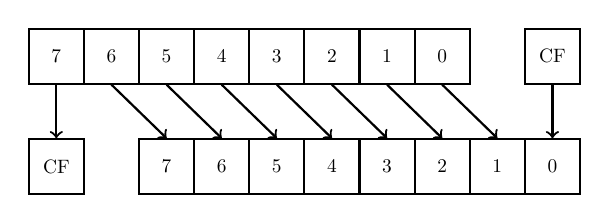
\begin{tikzpicture}[scale=0.7, every node/.style={scale=0.7}]
	\edef\bitsize{1cm}
	\tikzstyle{byte}=[draw,minimum size=\bitsize]
	\tikzstyle{every path}=[thick]

	\node [draw,rectangle,minimum size=\bitsize] (a1) {7};
	\node [draw,rectangle,minimum size=\bitsize] (a2) [right of=a1] {6};
	\node [draw,rectangle,minimum size=\bitsize] (a3) [right of=a2] {5};
	\node [draw,rectangle,minimum size=\bitsize] (a4) [right of=a3] {4};
	\node [draw,rectangle,minimum size=\bitsize] (a5) [right of=a4] {3};
	\node [draw,rectangle,minimum size=\bitsize] (a6) [right of=a5] {2};
	\node [draw,rectangle,minimum size=\bitsize] (a7) [right of=a6] {1};
	\node [draw,rectangle,minimum size=\bitsize] (a8) [right of=a7] {0};
	\node (empty1) [right of=a8] {};
	\node [rectangle,draw,minimum size=\bitsize] (acf) [right of=empty1] {CF};

	\node (empty) [below of=a1] {};

	\node [rectangle,draw,minimum size=\bitsize] (bcf) [below of=empty] {CF};
	\node (empty2) [right of=bcf] {};
	\node [draw,rectangle,minimum size=\bitsize] (b1) [right of=empty2] {7};
	\node [draw,rectangle,minimum size=\bitsize] (b2) [right of=b1] {6};
	\node [draw,rectangle,minimum size=\bitsize] (b3) [right of=b2] {5};
	\node [draw,rectangle,minimum size=\bitsize] (b4) [right of=b3] {4};
	\node [draw,rectangle,minimum size=\bitsize] (b5) [right of=b4] {3};
	\node [draw,rectangle,minimum size=\bitsize] (b6) [right of=b5] {2};
	\node [draw,rectangle,minimum size=\bitsize] (b7) [right of=b6] {1};
	\node [draw,rectangle,minimum size=\bitsize] (b8) [right of=b7] {0};

	\draw [->] (a1.south) -- (bcf.north); % 7
	\draw [->] (a2.south) -- (b1.north); % 6
	\draw [->] (a3.south) -- (b2.north);
	\draw [->] (a4.south) -- (b3.north);
	\draw [->] (a5.south) -- (b4.north);
	\draw [->] (a6.south) -- (b5.north);
	\draw [->] (a7.south) -- (b6.north);
	\draw [->] (a8.south) -- (b7.north);
	\draw [->] (acf.south) -- (b8.north);

	\end{tikzpicture}
\end{center}

  \item[RCR] (M) \RU{вращать биты направо через флаг CF}\EN{rotate right via CF flag}\FR{pivote vers la droite via le flag CF}:

\begin{center}
	\begin{tikzpicture}[scale=0.7, every node/.style={scale=0.7}]
	\edef\bitsize{1cm}
	\tikzstyle{byte}=[draw,minimum size=\bitsize]
	\tikzstyle{every path}=[thick]

	\node [rectangle,draw,minimum size=\bitsize] (acf) {CF};
	\node (empty1) [right of=acf] {};

	\node [draw,rectangle,minimum size=\bitsize] (a1) [right of=empty1] {7};
	\node [draw,rectangle,minimum size=\bitsize] (a2) [right of=a1] {6};
	\node [draw,rectangle,minimum size=\bitsize] (a3) [right of=a2] {5};
	\node [draw,rectangle,minimum size=\bitsize] (a4) [right of=a3] {4};
	\node [draw,rectangle,minimum size=\bitsize] (a5) [right of=a4] {3};
	\node [draw,rectangle,minimum size=\bitsize] (a6) [right of=a5] {2};
	\node [draw,rectangle,minimum size=\bitsize] (a7) [right of=a6] {1};
	\node [draw,rectangle,minimum size=\bitsize] (a8) [right of=a7] {0};

	\node (empty) [below of=a1] {};

	\node [draw,rectangle,minimum size=\bitsize] (b1) [below of=empty] {7};
	\node [draw,rectangle,minimum size=\bitsize] (b2) [right of=b1] {6};
	\node [draw,rectangle,minimum size=\bitsize] (b3) [right of=b2] {5};
	\node [draw,rectangle,minimum size=\bitsize] (b4) [right of=b3] {4};
	\node [draw,rectangle,minimum size=\bitsize] (b5) [right of=b4] {3};
	\node [draw,rectangle,minimum size=\bitsize] (b6) [right of=b5] {2};
	\node [draw,rectangle,minimum size=\bitsize] (b7) [right of=b6] {1};
	\node [draw,rectangle,minimum size=\bitsize] (b8) [right of=b7] {0};

	\node (empty2) [right of=b7] {};

	\node [rectangle,draw,minimum size=\bitsize] (bcf) [right=of empty2] {CF};

	\draw [->] (acf.south) -- (b1.north);
	\draw [->] (a1.south) -- (b2.north);
	\draw [->] (a2.south) -- (b3.north);
	\draw [->] (a3.south) -- (b4.north);
	\draw [->] (a4.south) -- (b5.north);
	\draw [->] (a5.south) -- (b6.north);
	\draw [->] (a6.south) -- (b7.north);
	\draw [->] (a7.south) -- (b8.north);
	\draw [->] (a8.south) -- (bcf.north);

	\end{tikzpicture}
\end{center}


\myindex{x86!\Instructions!ROL}
\myindex{x86!\Instructions!ROR}
\label{ROL_ROR}
\item[ROL/ROR] (M) \RU{циклический сдвиг}\EN{cyclic shift}
  
ROL: \RU{вращать налево}\EN{rotate left}:

\input{rotate_left}

ROR: \RU{вращать направо}\EN{rotate right}:

\input{rotate_right}

\RU{Не смотря на то что многие \ac{CPU} имеют эти инструкции, в \CCpp нет соответствующих операций,
так что компиляторы с этих \ac{PL} обычно не генерируют код использующий эти инструкции}\EN{Despite the 
fact that almost all \ac{CPU}s have these instructions, there are no corresponding
operations in \CCpp, so the compilers of these \ac{PL}s usually do not generate these 
instructions}.

\RU{Чтобы программисту были доступны эти инструкции, в \ac{MSVC} есть псевдофункции}
\EN{For the programmer's convenience, at least \ac{MSVC} has the pseudofunctions} (compiler intrinsics)
\emph{\_rotl()} \AndENRU \emph{\_rotr()}\FNMSDNROTxURL{},
\RU{которые транслируются компилятором напрямую в эти инструкции}
\EN{which are translated by the compiler directly to these instructions}.


\myindex{x86!\Instructions!SAL}
  \item[SAL] \RU{Арифметический сдвиг влево}\EN{Arithmetic shift left}\FR{Décalage
  arithmétique à gauche}, \RU{синонимично}\EN{synonymous to}\FR{synonyme de} \TT{SHL}

\myindex{x86!\Instructions!SAR}
  \label{ins:SAR}
  \item[SAR] \RU{Арифметический сдвиг вправо}\EN{Arithmetic shift right}\FR{Décalage arithmétique à droite}

\begin{center}
	\begin{tikzpicture}[scale=0.7, every node/.style={scale=0.7}]
	\edef\bitsize{1cm}
	\tikzstyle{byte}=[draw,minimum size=\bitsize]
	\tikzstyle{every path}=[thick]

	\node [draw,rectangle,minimum size=\bitsize] (a1) {7};
	\node [draw,rectangle,minimum size=\bitsize] (a2) [right of=a1] {6};
	\node [draw,rectangle,minimum size=\bitsize] (a3) [right of=a2] {5};
	\node [draw,rectangle,minimum size=\bitsize] (a4) [right of=a3] {4};
	\node [draw,rectangle,minimum size=\bitsize] (a5) [right of=a4] {3};
	\node [draw,rectangle,minimum size=\bitsize] (a6) [right of=a5] {2};
	\node [draw,rectangle,minimum size=\bitsize] (a7) [right of=a6] {1};
	\node [draw,rectangle,minimum size=\bitsize] (a8) [right of=a7] {0};

	\node (empty) [below of=a1] {};

	\node [draw,rectangle,minimum size=\bitsize] (b1) [below of=empty] {7};
	\node [draw,rectangle,minimum size=\bitsize] (b2) [right of=b1] {6};
	\node [draw,rectangle,minimum size=\bitsize] (b3) [right of=b2] {5};
	\node [draw,rectangle,minimum size=\bitsize] (b4) [right of=b3] {4};
	\node [draw,rectangle,minimum size=\bitsize] (b5) [right of=b4] {3};
	\node [draw,rectangle,minimum size=\bitsize] (b6) [right of=b5] {2};
	\node [draw,rectangle,minimum size=\bitsize] (b7) [right of=b6] {1};
	\node [draw,rectangle,minimum size=\bitsize] (b8) [right of=b7] {0};

	\node [shape=rectangle,draw,minimum size=\bitsize] (cf) [right=of b7] {CF};

	\draw [->] (a1.south) -- (b1.north); %7
	\draw [->] (a1.south) -- (b2.north); %6

	\draw [->] (a2.south) -- (b3.north); %6
	\draw [->] (a3.south) -- (b4.north); %5
	\draw [->] (a4.south) -- (b5.north); %4
	\draw [->] (a5.south) -- (b6.north); %3
	\draw [->] (a6.south) -- (b7.north); %2
	\draw [->] (a7.south) -- (b8.north); %1

	\draw [->] (a8.south) -- (cf.north);

	\end{tikzpicture}
\end{center}

\RU{Таким образом, бит знака всегда остается на месте}%
\EN{Hence, the sign bit always stays at the place of the}%
\FR{De ce fait, le bit de signe reste toujours à la place du} \ac{MSB}.


\myindex{x86!\Instructions!SETcc}
  \item[SETcc] op: \RU{загрузить 1 в op (только байт) если условие верно или 0 если наоборот}%
  \EN{load 1 to operand (byte only) if the condition is true or zero otherwise}%
  \FR{charge 1 dans l'opérande (octet seulement) si la condition est vraie et zéro sinon}.
  \RU{Коды точно такие же, как и в инструкциях Jcc}\EN{The condition codes are the same as in the Jcc instructions}%
  \FR{Les codes conditions sont les même que les instructions Jcc}
  (\myref{Jcc}).


\myindex{x86!\Instructions!STC}
\myindex{x86!\Flags!CF}
  \item[STC] (M) \RU{установить флаг CF}\EN{set CF flag}\FR{met le flag CF}

\input{appendix/x86/instructions/STD}
\myindex{x86!\Instructions!STI}
\myindex{x86!\Flags!IF}
  \item[STI] (M) \RU{установить флаг IF}\EN{set IF flag}\FR{met le flag IF}

\myindex{x86!\Instructions!SYSCALL}
  \item[SYSCALL] (AMD) \RU{вызов сисколла}\EN{call syscall}\FR{appelle un appel système} (\myref{syscalls})

\myindex{x86!\Instructions!SYSENTER}
  \item[SYSENTER] (Intel) \RU{вызов сисколла}\EN{call syscall}\FR{appel un appel système} (\myref{syscalls})

\myindex{x86!\Instructions!UD2}
  \item[UD2] (M) \RU{неопределенная инструкция, вызывает исключение. Применяется для тестирования.}
  \EN{undefined instruction, raises exception. Used for testing.}\FR{instruction
  indéfinie, lève une exception. Utilisée pour tester.}

\myindex{x86!\Instructions!XCHG}
  \item[XCHG] (M) \RU{обменять местами значения в операндах}\EN{exchange the values in the operands}%
\FR{échange les valeurs dans les opérandes}

\myindex{Borland Delphi}
\RU{Это редкая инструкция: компиляторы её не генерируют, потому что начиная с Pentium, XCHG с адресом в памяти в операнде
исполняется так, как если имеет префикс LOCK (см.\InSqBrackets{\MAbrash глава 19}).
Вероятно, в Intel так сделали для совместимости с синхронизирующими примитивами.
Таким образом, XCHG начиная с Pentium может быть медленной.
С другой стороны, XCHG была очень популярна у программистов на ассемблере.
Так что, если вы видите XCHG в коде, это может быть знаком, что код написан вручную.
Впрочем, по крайней мере компилятор Borland Delphi генерирует эту инструкцию.}
\EN{This instruction is rare: compilers don't generate it, because starting at Pentium, XCHG with address in memory in operand executes as if it has LOCK prefix (\InSqBrackets{\MAbrash chapter 19}).
Perhaps, Intel engineers did so for compatibility with synchronizing primitives.
Hence, XCHG starting at Pentium can be slow.
On the other hand, XCHG was very popular in assembly language programmers.
So if you see XCHG in code, it can be a sign that this piece of code is written manually.
However, at least Borland Delphi compiler generates this instruction.}
\FR{Cette instruction est rare: les compilateurs ne la génère pas, car à partir du
Pentium, XCHG avec comme opérande une adresse en mémoire s'exécute comme si elle
avait le préfixe LOCK (\InSqBrackets{\MAbrash chapter 19}).
Peut-être que les ingénieurs d'Intel ont fait cela pour la compatibilité avec les
primitives de synchronisation.
Ainsi, à partir du Pentium, XCHG peut être lente.
D'un autre côté, XCHG était très populaire chez les programmeurs en langage d'assemblage.
Donc, si vous voyez XCHG dans le code, ça peut être un signe que ce morceau de code
a été écrit à la main.
Toutefois, au moins le compilateur Borland Delphi génère cette instruction.}


\end{description}

\subsubsection{\RU{Инструкции FPU}\EN{FPU instructions}}

\RU{Суффикс \TT{-R} в названии инструкции обычно означает, что операнды поменяны местами, суффикс \TT{-P} означает
что один элемент выталкивается из стека после исполнения инструкции, суффикс \TT{-PP} означает, что
выталкиваются два элемента}%
\EN{\TT{-R} suffix in the mnemonic usually implies that the operands are reversed,
\TT{-P} suffix implies that one element is popped
from the stack after the instruction's execution, \TT{-PP} suffix implies that two elements are popped}.

\TT{-P} \RU{инструкции часто бывают полезны, когда нам уже больше не нужно хранить значение в 
FPU-стеке после операции.}%
\EN{instructions are often useful when we do not need the value in the FPU stack to be 
present anymore after the operation.}

\begin{description}
\myindex{x86!\Instructions!FABS}
  \item[FABS] \RU{заменить значение в ST(0) на абсолютное значение ST(0)}\EN{replace value in ST(0) by absolute value in ST(0)}%
  \FR{remplace la valeur dans ST(0) par sa valeur absolue}

\myindex{x86!\Instructions!FADD}
\myindex{x86!\Instructions!FADDP}
  \item[FADD] op: ST(0)=op+ST(0)
  \item[FADD] ST(0), ST(i): ST(0)=ST(0)+ST(i)
  \item[FADDP] ST(1)=ST(0)+ST(1);
  \RU{вытолкнуть один элемент из стека, таким образом, складываемые значения в стеке заменяются
  суммой}\EN{pop one element from the stack, i.e., the values in the stack are replaced by their sum}%
  \FR{supprime un élément de la pile, i.e., les valeurs sur la pile sont remplacées par leurs somme}

 % + FADDP
\input{appendix/x86/instructions/FCHS}
\input{appendix/x86/instructions/FCOM} % + FCOMP + FCOMPP
\myindex{x86!\Instructions!FDIVR}
\myindex{x86!\Instructions!FDIVRP}
  \item[FDIVR] op: ST(0)=op/ST(0)
  \item[FDIVR] ST(i), ST(j): ST(i)=ST(j)/ST(i)
  \item[FDIVRP] op: ST(0)=op/ST(0); \RU{вытолкнуть один элемент из стека}\EN{pop one element from the stack}%
  \FR{supprime un élément de la pile}
  \item[FDIVRP] ST(i), ST(j): ST(i)=ST(j)/ST(i); \RU{вытолкнуть один элемент из стека}\EN{pop one element from the stack}%
  \FR{supprime un élément de la pile}

 % + FDIVRP
\myindex{x86!\Instructions!FDIV}
\myindex{x86!\Instructions!FDIVP}
  \item[FDIV] op: ST(0)=ST(0)/op
  \item[FDIV] ST(i), ST(j): ST(i)=ST(i)/ST(j)
  \item[FDIVP] ST(1)=ST(0)/ST(1); \RU{вытолкнуть один элемент из стека, таким образом,
  делимое и делитель в стеке заменяются частным}\EN{pop one element from the stack, i.e.,
  the dividend and divisor values in the stack are replaced by quotient}\FR{supprime un
  élément de la pile, i.e, les valeurs du dividende et du diviseur sont remplacées par
  le quotient}
 % + FDIVP
\myindex{x86!\Instructions!FILD}
  \item[FILD] op: \RU{сконвертировать целочисленный op и затолкнуть его в стек}
  \EN{convert integer and push it to the stack}\FR{convertit un entier n et le pousse sur la pile}.


\input{appendix/x86/instructions/FIST} % + FISTP
\myindex{x86!\Instructions!FLD1}
  \item[FLD1] \RU{затолкнуть 1 в стек}\EN{push 1 to stack}\FR{pousse 1 sur la pile}


\myindex{x86!\Instructions!FLDCW}
  \item[FLDCW] op: \RU{загрузить}\EN{load}\FR{charge le} FPU control word (\myref{FPU_control_word}) \RU{из}\EN{from}\FR{depuis le} 16-bit op.


\myindex{x86!\Instructions!FLDZ}
  \item[FLDZ] \RU{затолкнуть ноль в стек}\EN{push zero to stack}\FR{pousse zéro sur la pile}



\myindex{x86!\Instructions!FLD}
  \item[FLD] op: \RU{затолкнуть op в стек}\EN{push op to the stack}\FR{pousse op sur la pile}.

\myindex{x86!\Instructions!FMUL}
\myindex{x86!\Instructions!FMULP}
  \item[FMUL] op: ST(0)=ST(0)*op
  \item[FMUL] ST(i), ST(j): ST(i)=ST(i)*ST(j)
  \item[FMULP] op: ST(0)=ST(0)*op; \RU{вытолкнуть один элемент из стека}\EN{pop one element from the stack}%
  \FR{supprime un élément de la pile}
  \item[FMULP] ST(i), ST(j): ST(i)=ST(i)*ST(j); \RU{вытолкнуть один элемент из стека}\EN{pop one element from the stack}%
  \FR{supprime un élément de la pile}

 % + FMULP
\input{appendix/x86/instructions/FSINCOS}
\input{appendix/x86/instructions/FSQRT}
\input{appendix/x86/instructions/FSTCW} % + FNSTCW
\input{appendix/x86/instructions/FSTSW} % + FNSTSW
\myindex{x86!\Instructions!FST}
\myindex{x86!\Instructions!FSTP}
  \item[FST] op: \RU{копировать}\EN{copy}\FR{copie} ST(0) \RU{в}\EN{to}\FR{dans} op
  \item[FSTP] op: \RU{копировать}\EN{copy}\FR{copie} ST(0) \RU{в}\EN{to}\FR{dans} op;
  \RU{вытолкнуть один элемент из стека}\EN{pop one element from the stack}%
  \FR{supprime un élément de la pile}

\myindex{x86!\Instructions!FSUBR}
\myindex{x86!\Instructions!FSUBRP}
  \item[FSUBR] op: ST(0)=op-ST(0)
  \item[FSUBR] ST(0), ST(i): ST(0)=ST(i)-ST(0)
  \item[FSUBRP] ST(1)=ST(0)-ST(1);
  \RU{вытолкнуть один элемент из стека, таким образом, складываемые значения в стеке заменяются
  разностью}\EN{pop one element from the stack, i.e., the value in the stack is replaced by the difference}%
  \FR{supprime un élément de la pile, i.e., la valeur dans la pile est remplacée par la différence}

 % + FSUBRP
\myindex{x86!\Instructions!FSUB}
\myindex{x86!\Instructions!FSUBP}
  \item[FSUB] op: ST(0)=ST(0)-op
  \item[FSUB] ST(0), ST(i): ST(0)=ST(0)-ST(i)
  \item[FSUBP] ST(1)=ST(1)-ST(0);
  \RU{вытолкнуть один элемент из стека, таким образом, складываемые значения в стеке заменяются
  разностью}\EN{pop one element from the stack, i.e., the value in the stack is replaced by the difference}%
  \FR{supprime un élément de la pile, i.e., la valeur dans la pile est remplacée par la différence}

 % + FSUBP
\input{appendix/x86/instructions/FUCOM} % + FUCOMP + FUCOMPP
\myindex{x86!\Instructions!FXCH}
  \item[FXCH] ST(i) \RU{обменять местами значения в ST(0) и ST(i)}\EN{exchange values in ST(0) and ST(i)}%
  \FR{échange les valeurs dans ST(0) et ST(i)}
  \item[FXCH] \RU{обменять местами значения в ST(0) и ST(1)}\EN{exchange values in ST(0) and ST(1)}%
  \FR{échange les valeurs dans ST(0) et ST(1)}


\end{description}

%\subsubsection{\RU{SIMD-инструкции}\EN{SIMD instructions}}

% TODO

%\begin{description}
%\input{appendix/x86/instructions/DIVSD}
%\input{appendix/x86/instructions/MOVDQA}
%\input{appendix/x86/instructions/MOVDQU}
%\input{appendix/x86/instructions/PADDD}
%\input{appendix/x86/instructions/PCMPEQB}
%\input{appendix/x86/instructions/PLMULHW}
%\input{appendix/x86/instructions/PLMULLD}
%\input{appendix/x86/instructions/PMOVMSKB}
%\input{appendix/x86/instructions/PXOR}
%\end{description}

% SHLD !
% SHRD !
% BSWAP !
% CMPXCHG
% XADD !
% CMPXCHG8B
% RDTSC !
% PAUSE!

% xsave
% fnclex, fnsave
% movsxd, movaps, wait, sfence, lfence, pushfq
% prefetchw
% REP RETN
% REP BSF
% movnti, movntdq, rdmsr, wrmsr
% ldmxcsr, stmxcsr, invlpg
% swapgs
% movq, movd
% mulsd
% POR
% IRETQ
% pslldq
% psrldq
% cqo, fxrstor, comisd, xrstor, wbinvd, movntq
% fprem
% addsb, subsd, frndint

% rare:
%\item[ENTER]
%\item[LES]
% LDS
% XLAT

\subsubsection{\RU{Инструкции с печатаемым ASCII-опкодом}\EN{Instructions having printable ASCII opcode}}

(\RU{В 32-битном режиме}\EN{In 32-bit mode}).

\label{printable_x86_opcodes}
\myindex{Shellcode}
\RU{Это может пригодиться для создания шеллкодов}\EN{These can be suitable for shellcode construction}.
\RU{См. также}\EN{See also}: \myref{subsec:EICAR}.

% FIXME: start at 0x20...
\begin{center}
\begin{longtable}{ | l | l | l | }
\hline
\HeaderColor ASCII\RU{-символ}\EN{ character} & 
\HeaderColor \RU{шестнадцатеричный код}\EN{hexadecimal code} & 
\HeaderColor x86\RU{-инструкция}\EN{ instruction} \\
\hline
0	 &30	 &XOR \\
1	 &31	 &XOR \\
2	 &32	 &XOR \\
3	 &33	 &XOR \\
4	 &34	 &XOR \\
5	 &35	 &XOR \\
7	 &37	 &AAA \\
8	 &38	 &CMP \\
9	 &39	 &CMP \\
:	 &3a	 &CMP \\
;	 &3b	 &CMP \\
<	 &3c	 &CMP \\
=	 &3d	 &CMP \\
?	 &3f	 &AAS \\
@	 &40	 &INC \\
A	 &41	 &INC \\
B	 &42	 &INC \\
C	 &43	 &INC \\
D	 &44	 &INC \\
E	 &45	 &INC \\
F	 &46	 &INC \\
G	 &47	 &INC \\
H	 &48	 &DEC \\
I	 &49	 &DEC \\
J	 &4a	 &DEC \\
K	 &4b	 &DEC \\
L	 &4c	 &DEC \\
M	 &4d	 &DEC \\
N	 &4e	 &DEC \\
O	 &4f	 &DEC \\
P	 &50	 &PUSH \\
Q	 &51	 &PUSH \\
R	 &52	 &PUSH \\
S	 &53	 &PUSH \\
T	 &54	 &PUSH \\
U	 &55	 &PUSH \\
V	 &56	 &PUSH \\
W	 &57	 &PUSH \\
X	 &58	 &POP \\
Y	 &59	 &POP \\
Z	 &5a	 &POP \\
\lbrack{}	 &5b	 &POP \\
\textbackslash{}	 &5c	 &POP \\
\rbrack{}	 &5d	 &POP \\
\verb|^|	 &5e	 &POP \\
\_	 &5f	 &POP \\
\verb|`|	 &60	 &PUSHA \\
a	 &61	 &POPA \\

h	 &68	 &PUSH\\
i	 &69	 &IMUL\\
j	 &6a	 &PUSH\\
k	 &6b	 &IMUL\\
p	 &70	 &JO\\
q	 &71	 &JNO\\
r	 &72	 &JB\\
s	 &73	 &JAE\\
t	 &74	 &JE\\
u	 &75	 &JNE\\
v	 &76	 &JBE\\
w	 &77	 &JA\\
x	 &78	 &JS\\
y	 &79	 &JNS\\
z	 &7a	 &JP\\
\hline
\end{longtable}
\end{center}

\RU{А также}\EN{Also}:

\begin{center}
\begin{longtable}{ | l | l | l | }
\hline
\HeaderColor ASCII\RU{-символ}\EN{ character} & 
\HeaderColor \RU{шестнадцатеричный код}\EN{hexadecimal code} & 
\HeaderColor x86\RU{-инструкция}\EN{ instruction} \\
\hline
f	 &66	 &\RU{(в 32-битном режиме) переключиться на}\EN{(in 32-bit mode) switch to}\\
   & & \RU{16-битный размер операнда}\EN{16-bit operand size} \\
g	 &67	 &\RU{(в 32-битном режиме) переключиться на}\EN{in 32-bit mode) switch to}\\
   & & \RU{16-битный размер адреса}\EN{16-bit address size} \\
\hline
\end{longtable}
\end{center}

\myindex{x86!\Instructions!AAA}
\myindex{x86!\Instructions!AAS}
\myindex{x86!\Instructions!CMP}
\myindex{x86!\Instructions!DEC}
\myindex{x86!\Instructions!IMUL}
\myindex{x86!\Instructions!INC}
\myindex{x86!\Instructions!JA}
\myindex{x86!\Instructions!JAE}
\myindex{x86!\Instructions!JB}
\myindex{x86!\Instructions!JBE}
\myindex{x86!\Instructions!JE}
\myindex{x86!\Instructions!JNE}
\myindex{x86!\Instructions!JNO}
\myindex{x86!\Instructions!JNS}
\myindex{x86!\Instructions!JO}
\myindex{x86!\Instructions!JP}
\myindex{x86!\Instructions!JS}
\myindex{x86!\Instructions!POP}
\myindex{x86!\Instructions!POPA}
\myindex{x86!\Instructions!PUSH}
\myindex{x86!\Instructions!PUSHA}
\myindex{x86!\Instructions!XOR}

\RU{В итоге}\EN{In summary}:
AAA, AAS, CMP, DEC, IMUL, INC, JA, JAE, JB, JBE, JE, JNE, JNO, JNS, JO, JP, JS, POP, POPA, PUSH, PUSHA, 
XOR.

 % subsection
\subsection{npad}
\label{sec:npad}

\RU{Это макрос в ассемблере, для выравнивания некоторой метки по некоторой границе.}
\EN{It is an assembly language macro for aligning labels on a specific boundary.}
\DE{Dies ist ein Assembler-Makro um Labels an bestimmten Grenzen auszurichten.}
\FR{C'est une macro du langage d'assemblage pour aligner les labels sur une limite
spécifique.}

\RU{Это нужно для тех \emph{нагруженных} меток, куда чаще всего передается управление, например, 
начало тела цикла. 
Для того чтобы процессор мог эффективнее вытягивать данные или код из памяти, через шину с памятью, 
кэширование, итд.}
\EN{That's often needed for the busy labels to where the control flow is often passed, e.g., loop body starts.
So the CPU can load the data or code from the memory effectively, through the memory bus, cache lines, etc.}
\DE{Dies ist oft nützlich Labels, die oft Ziel einer Kotrollstruktur sind, wie Schleifenköpfe.
Somit kann die CPU Daten oder Code sehr effizient vom Speicher durch den Bus, den Cache, usw. laden.}
\FR{C'est souvent nécessaire pour des labels très utilisés, comme par exemple le
début d'un corps de boucle. Ainsi, le CPU peut charger les données ou le code depuis
la mémoire efficacement, à travers le bus mémoire, les caches, etc.}

\RU{Взято из}\EN{Taken from}\DE{Entnommen von}\FR{Pris de} \TT{listing.inc} (MSVC):

\myindex{x86!\Instructions!NOP}
\RU{Это, кстати, любопытный пример различных вариантов \NOP{}-ов. 
Все эти инструкции не дают никакого эффекта, но отличаются разной длиной.}
\EN{By the way, it is a curious example of the different \NOP variations.
All these instructions have no effects whatsoever, but have a different size.}
\DE{Dies ist übrigens ein Beispiel für die unterschiedlichen \NOP-Variationen.
Keine dieser Anweisungen hat eine Auswirkung, aber alle haben eine unterschiedliche Größe.}
\FR{À propos, c'est un exemple curieux des différentes variations de \NOP. Toutes
ces instructions n'ont pas d'effet, mais ont une taille différente.}

\RU{Цель в том, чтобы была только одна инструкция, а не набор NOP-ов, 
считается что так лучше для производительности CPU.}
\EN{Having a single idle instruction instead of couple of NOP-s,
is accepted to be better for CPU performance.}
\DE{Eine einzelne Idle-Anweisung anstatt mehrerer NOPs hat positive Auswirkungen
auf die CPU-Performance.}
\FR{Avoir une seule instruction sans effet au lieu de plusieurs est accepté comme
étant meilleur pour la performance du CPU.}

\begin{lstlisting}[style=customasmx86]
;; LISTING.INC
;;
;; This file contains assembler macros and is included by the files created
;; with the -FA compiler switch to be assembled by MASM (Microsoft Macro
;; Assembler).
;;
;; Copyright (c) 1993-2003, Microsoft Corporation. All rights reserved.

;; non destructive nops
npad macro size
if size eq 1
  nop
else
 if size eq 2
   mov edi, edi
 else
  if size eq 3
    ; lea ecx, [ecx+00]
    DB 8DH, 49H, 00H
  else
   if size eq 4
     ; lea esp, [esp+00]
     DB 8DH, 64H, 24H, 00H
   else
    if size eq 5
      add eax, DWORD PTR 0
    else
     if size eq 6
       ; lea ebx, [ebx+00000000]
       DB 8DH, 9BH, 00H, 00H, 00H, 00H
     else
      if size eq 7
	; lea esp, [esp+00000000]
	DB 8DH, 0A4H, 24H, 00H, 00H, 00H, 00H 
      else
       if size eq 8
        ; jmp .+8; .npad 6
	DB 0EBH, 06H, 8DH, 9BH, 00H, 00H, 00H, 00H
       else
        if size eq 9
         ; jmp .+9; .npad 7
         DB 0EBH, 07H, 8DH, 0A4H, 24H, 00H, 00H, 00H, 00H
        else
         if size eq 10
          ; jmp .+A; .npad 7; .npad 1
          DB 0EBH, 08H, 8DH, 0A4H, 24H, 00H, 00H, 00H, 00H, 90H
         else
          if size eq 11
           ; jmp .+B; .npad 7; .npad 2
           DB 0EBH, 09H, 8DH, 0A4H, 24H, 00H, 00H, 00H, 00H, 8BH, 0FFH
          else
           if size eq 12
            ; jmp .+C; .npad 7; .npad 3
            DB 0EBH, 0AH, 8DH, 0A4H, 24H, 00H, 00H, 00H, 00H, 8DH, 49H, 00H
           else
            if size eq 13
             ; jmp .+D; .npad 7; .npad 4
             DB 0EBH, 0BH, 8DH, 0A4H, 24H, 00H, 00H, 00H, 00H, 8DH, 64H, 24H, 00H
            else
             if size eq 14
              ; jmp .+E; .npad 7; .npad 5
              DB 0EBH, 0CH, 8DH, 0A4H, 24H, 00H, 00H, 00H, 00H, 05H, 00H, 00H, 00H, 00H
             else
              if size eq 15
               ; jmp .+F; .npad 7; .npad 6
               DB 0EBH, 0DH, 8DH, 0A4H, 24H, 00H, 00H, 00H, 00H, 8DH, 9BH, 00H, 00H, 00H, 00H
              else
	       %out error: unsupported npad size
               .err
              endif
             endif
            endif
           endif
          endif
         endif
        endif
       endif
      endif
     endif
    endif
   endif
  endif
 endif
endif
endm
\end{lstlisting}
 % subsection

